%%%%%%%%%%%%%%%%%%%%%%%%%%%%%%%%%%%%%%%%%%%%%%%%%%%%
% Document type, global settings, and packages
%%%%%%%%%%%%%%%%%%%%%%%%%%%%%%%%%%%%%%%%%%%%%%%%%%%%

\documentclass[12pt]{report}   %12 point font for Times New Roman
\usepackage{graphicx}  %for images and plots
\usepackage[letterpaper, left=1.5in, right=1in, top=1in, bottom=1in]{geometry}
\usepackage{setspace}  %use this package to set linespacing as desired
\usepackage{times}  %set Times New Roman as the font
\usepackage[explicit]{titlesec}  %title control and formatting
\usepackage[titles]{tocloft}  %table of contents control and formatting
\usepackage[backend=bibtex, sorting=none, bibstyle=ieee]{biblatex}  %reference manager
\usepackage[bookmarks=true, hidelinks]{hyperref}
\usepackage[page]{appendix}  %for appendices
\usepackage{rotating}  %for rotated, landscape images
\usepackage[normalem]{ulem}  %for italicized text
\usepackage{amsmath}
\usepackage{algorithm}
\usepackage{algorithmic}
\usepackage{float}
\usepackage{subfig}
\usepackage[symbol]{footmisc}

%%%%%%%%%%%%%%%%%%%%%%%%%%%%%%%%%%%
% Bibliography
%%%%%%%%%%%%%%%%%%%%%%%%%%%%%%%%%%%

%Add your bibliography file here
\bibliography{references}

% prevent certain fields in references from printing in bibliography
\AtEveryBibitem{\clearfield{issn}}
\AtEveryBibitem{\clearlist{issn}}

\AtEveryBibitem{\clearfield{language}}
\AtEveryBibitem{\clearlist{language}}

\AtEveryBibitem{\clearfield{doi}}
\AtEveryBibitem{\clearlist{doi}}

\AtEveryBibitem{\clearfield{url}}
\AtEveryBibitem{\clearlist{url}}

\AtEveryBibitem{%
  \ifentrytype{online}
    {}
    {\clearfield{urlyear}\clearfield{urlmonth}\clearfield{urlday}}}

%%%%%%%%%%%%%%%%%%%%%%
% Start of Document
%%%%%%%%%%%%%%%%%%%%%%

\begin{document}
\doublespacing  %set line spacing

%%%%%%%%%%%%%%%%%%%%%%%%%%%%%%%%%%%%%
% Title Page
%%%%%%%%%%%%%%%%%%%%%%%%%%%%%%%%%%%%%

%% Define your thesis title, your name, your school, and your month and year of graduation here

\newcommand{\thesisTitle}{Optimizing Computational Kernels in Quantum Chemistry}
\newcommand{\yourName}{Matthew C. Schieber}
\newcommand{\yourSchool}{Computational Science and Engineering}
\newcommand{\yourMonth}{March}
\newcommand{\yourYear}{2018}

%%%%%%%%%%%%%%%%%%%%%%%%%%%%%%%%%%%%%%%%%%%%%%%%%%%%%%%%%
% Do not edit these lines unless you wish to customize
% the template
%%%%%%%%%%%%%%%%%%%%%%%%%%%%%%%%%%%%%%%%%%%%%%%%%%%%%%%%%



\begin{titlepage}
\begin{center}

\begin{singlespacing}

\textbf{\MakeUppercase{\thesisTitle}}\\
\vspace{10\baselineskip}
A Thesis\\
Presented to\\
The Academic Faculty\\
\vspace{3\baselineskip}
By\\
\vspace{3\baselineskip}
\yourName\\
\vspace{3\baselineskip}
In Partial Fulfillment\\
of the Requirements for the Degree\\
Master of Science in the\\
School of \yourSchool\\
\vspace{3\baselineskip}
Georgia Institute of Technology\\
\vspace{\baselineskip}
\yourMonth{} \yourYear{}
\vfill
Copyright \copyright{} \yourName{} \yourYear{}

\end{singlespacing}

\end{center}
\end{titlepage}



\currentpdfbookmark{Title Page}{titlePage}  %add PDF bookmark for this page

%%%%%%%%%%%%%%%%%%%%%%%%%%%%%%%%%%%%%
% Approval Page
%%%%%%%%%%%%%%%%%%%%%%%%%%%%%%%%%%%%%

%% Define your committee members. If you have less than 6, simple delete/comment the unused lines

\newcommand{\committeeMemberOne}{Dr. Sherrill, Advisor}
\newcommand{\committeeMemberOneDepartment}{School of Chemistry and Biochemistry, School of Computational Science and Engineering}
\newcommand{\committeeMemberOneAffiliation}{Georgia Institute of Technology}

\newcommand{\committeeMemberTwo}{Dr. Chow}
\newcommand{\committeeMemberTwoDepartment}{School of Computational Science and Engineering}
\newcommand{\committeeMemberTwoAffiliation}{Georgia Institute of Technology}

\newcommand{\committeeMemberThree}{Dr. McDaniel}
\newcommand{\committeeMemberThreeDepartment}{School of Chemistry and Biochemistry}
\newcommand{\committeeMemberThreeAffiliation}{Georgia Institute of Technology}

\newcommand{\approvalDay}{April 21, 2018}
\newcommand{\approvalMonth}{}
\newcommand{\approvalYear}{}

%%%%%%%%%%%%%%%%%%%%%%%%%%%%%%%%%%%%%%%%%%%%%%%%%%%%%%%%%
% Do not edit these lines unless you wish to customize
% the template
%%%%%%%%%%%%%%%%%%%%%%%%%%%%%%%%%%%%%%%%%%%%%%%%%%%%%%%%%


\begin{titlepage}
\begin{singlespacing}
\begin{center}

\textbf{\MakeUppercase{\thesisTitle}}\\
\vspace{10\baselineskip}

\end{center}
\vfill

%Define minipages, depending on how many authors there are
\ifdefined\committeeMemberFour

Approved by:
\vspace{2\baselineskip}		%adjust the number in front of "\baselineskip" for alignment

\begin{minipage}[b]{0.4\textwidth}
	
	\committeeMemberOne\\
	\committeeMemberOneDepartment\\
	\textit{\committeeMemberOneAffiliation}\\
	
	\committeeMemberTwo\\
	\committeeMemberTwoDepartment\\
	\textit{\committeeMemberTwoAffiliation}\\
	
	\committeeMemberThree\\
	\committeeMemberThreeDepartment\\
	\textit{\committeeMemberThreeAffiliation}\\
	
	\vspace{2\baselineskip}		%adjust the number in front of "\baselineskip" for alignment
	
\end{minipage}
\hspace{0.1\textwidth}
\begin{minipage}[b]{0.4\textwidth}
	
	\committeeMemberFour\\
	\committeeMemberFourDepartment\\
	\textit{\committeeMemberFourAffiliation}\\
	
	\ifdefined\committeeMemberSix
	\committeeMemberFive\\
	\committeeMemberFiveDepartment\\
	\textit{\committeeMemberFiveAffiliation}\\
	
	\committeeMemberSix\\
	\committeeMemberSixDepartment\\
	\textit{\committeeMemberSixAffiliation}\\
	
	Date Approved: \approvalMonth{} \approvalDay, \approvalYear
	\vspace{1\baselineskip}		%adjust the number in front of "\baselineskip" for alignment
	
	\else
	
	\committeeMemberFive\\
	\committeeMemberFiveDepartment\\
	\textit{\committeeMemberFiveAffiliation}\\
		
	Date Approved: \approvalMonth{} \approvalDay, \approvalYear
	\vspace{5\baselineskip}		%adjust the number in front of "\baselineskip" for alignment
	
	\fi
	
\end{minipage}

\else

\hspace{0.6\textwidth}
\begin{minipage}[b]{0.4\textwidth}
	
	Approved by:
	\vspace{2\baselineskip}		%adjust the number in front of "\baselineskip" for alignment
	
	\committeeMemberOne\\
	\committeeMemberOneDepartment\\
	\textit{\committeeMemberOneAffiliation}\\
	
	\committeeMemberTwo\\
	\committeeMemberTwoDepartment\\
	\textit{\committeeMemberTwoAffiliation}\\
	
	\committeeMemberThree\\
	\committeeMemberThreeDepartment\\
	\textit{\committeeMemberThreeAffiliation}\\
	
	\vspace{2\baselineskip}		%adjust the number in front of "\baselineskip" for alignment
	
	Date Approved: \approvalMonth{} \approvalDay, \approvalYear
	\vspace{\baselineskip}		%adjust the number in front of "\baselineskip" for alignment
	
\end{minipage}

\fi





\end{singlespacing}
\end{titlepage}


%%%%%%%%%%%%%%%%%%%%%%%%%%%%%%%%%%%%%
% Epigraph
%%%%%%%%%%%%%%%%%%%%%%%%%%%%%%%%%%%%%

%% Define your quote and author for the epigraph here

\newcommand{\yourQuote}{A great quote to start the thesis}
\newcommand{\yourAuthor}{George P. Burdell}

%%%%%%%%%%%%%%%%%%%%%%%%%%%%%%%%%%%%%%%%%%%%%%%%%%%%%%%%%
% Do not edit these lines unless you wish to customize
% the template
%%%%%%%%%%%%%%%%%%%%%%%%%%%%%%%%%%%%%%%%%%%%%%%%%%%%%%%%%

\begin{titlepage}
\begin{center}

\vspace*{\fill}
\yourQuote\\
\textit{\yourAuthor}
\vspace*{\fill}

\end{center}
\end{titlepage}



%%%%%%%%%%%%%%%%%%%%%%%%%%%%%%%%%%%%%
% Dedication
%%%%%%%%%%%%%%%%%%%%%%%%%%%%%%%%%%%%%

% Define your dedication statement here

\newcommand{\yourDedication}{To my mom and dad.}

%%%%%%%%%%%%%%%%%%%%%%%%%%%%%%%%%%%%%%%%%%%%%%%%%%%%%%%%%
% Do not edit these lines unless you wish to customize
% the template
%%%%%%%%%%%%%%%%%%%%%%%%%%%%%%%%%%%%%%%%%%%%%%%%%%%%%%%%%

\begin{titlepage}
\begin{center}

\vspace*{\fill}
\yourDedication\\
\vspace*{\fill}

\end{center}
\end{titlepage}


%%%%%%%%%%%%%%%%%%%%%%%%%%%%%%%%%%%%%
% Acknowledgments
%%%%%%%%%%%%%%%%%%%%%%%%%%%%%%%%%%%%%

\pagenumbering{roman}
\addcontentsline{toc}{chapter}{Acknowledgments}
\setcounter{page}{4} % set the page number appropriately based on the number of intro pages
\clearpage
\begin{centering}
\textbf{ACKNOWLEDGEMENTS}\\
\vspace{\baselineskip}
\end{centering}

%Insert your dedication text here

\noindent I would like to thank my parents, Mike and Trish, for their love and support throughout my life.
Thank you so much for instilling the curiousity and dedication in me which made this possible.
My sisters, brothers, nieces, nephews, and cousins deserve my appreciation as well.

\hfill

\noindent I would like to sincerely thank my supervisor, Prof. Sherrill, for his guidance and support.
His belief in me provided encouragement throughout this entire process. I would also like to
thank Dr. Chow for co-advising me. The insights I learned from his courses made much of this work
possible. Also, I would like to thank Dr. Smith, who, without his mentorship and guidance, none
of this would have been possible. Collaborating with him was truly inspiring.

\hfill

\noindent I greatly appreciate the support of groupmates within the Sherrill Lab. Brandon, thank you for
your superb automation skills and willingness to run tests for me. Lori, thank you for letting me bug you often about
how to compile Psi4. Thank you Dom, Assim, Constance, Carlos, and Yi for the support and fun times. 

\hfill

\noindent Last but not least, I would like to thank my girlfriend, Andrea, whose emotional and intellectual support
kept me above water throughout graduate school.


\clearpage
%\pagenumbering{gobble}  %remove page number on summary page


%\addtocontents{toc}{\cftpagenumbersoff{chapter}} 

%\currentpdfbookmark{Acknowledgments}{acknowledgments}
%\addtocontents{toc}{\cftpagenumberson{chapter}} 

%%%%%%%%%%%%%%%%%%%%%%%%%%%%%%%%%%%%%
% Table of Contents
%%%%%%%%%%%%%%%%%%%%%%%%%%%%%%%%%%%%%

% Format for Table of Contents
\renewcommand{\cftchapdotsep}{\cftdotsep}  %add dot separators
\renewcommand{\cftchapfont}{\bfseries}  %set title font weight
\renewcommand{\cftchappagefont}{}  %set page number font weight
\renewcommand{\cftchappresnum}{Chapter }
\renewcommand{\cftchapaftersnum}{:}
\renewcommand{\cftchapnumwidth}{5em}
\renewcommand{\cftchapafterpnum}{\vskip\baselineskip} %set correct spacing for entries in single space environment
\renewcommand{\cftsecafterpnum}{\vskip\baselineskip}  %set correct spacing for entries in single space environment
\renewcommand{\cftsubsecafterpnum}{\vskip\baselineskip} %set correct spacing for entries in single space environment
\renewcommand{\cftsubsubsecafterpnum}{\vskip\baselineskip} %set correct spacing for entries in single space environment

%format title font size and position (this also applys to list of figures and list of tables)
\titleformat{\chapter}[display]
{\normalfont\bfseries\filcenter}{\chaptertitlename\ \thechapter}{0pt}{\MakeUppercase{#1}}

\renewcommand\contentsname{Table of Contents}

\begin{singlespace}
\tableofcontents
\end{singlespace}

\currentpdfbookmark{Table of Contents}{TOC}

\clearpage

%%%%%%%%%%%%%%%%%%%%%%%%%%%%%%%%%%%%%
% List of figures and tables
%%%%%%%%%%%%%%%%%%%%%%%%%%%%%%%%%%%%%

\addcontentsline{toc}{chapter}{List of Tables}
\begin{singlespace}
	\setlength\cftbeforetabskip{\baselineskip}  %manually set spacing between entries
	\listoftables
\end{singlespace}

\clearpage

\addcontentsline{toc}{chapter}{List of Figures}
\begin{singlespace}
\setlength\cftbeforefigskip{\baselineskip}  %manually set spacing between entries
\listoffigures
\end{singlespace}

\clearpage

%%%%%%%%%%%%%%%%%%%%%%%%%%%%%%%%%%%%%%%%%%%%%%%%%%%%%%%%%%%%%%%%%
% This is the Summary (abstract should be separate document)
%%%%%%%%%%%%%%%%%%%%%%%%%%%%%%%%%%%%%%%%%%%%%%%%%%%%%%%%%%%%%%%%%

\clearpage
\begin{centering}
\textbf{SUMMARY}\\
\vspace{\baselineskip}
\end{centering}

Density fitting is a rank reduction technique popularly used in quantum chemistry in order to reduce the computational cost 
of evaluating, transforming, and processing the 4-center electron repulsion integrals (ERIs). By utilizing the resolution of the 
identity technique, density fitting reduces the 4-center ERIs into a 3-center form. Doing so not only alleviates the high storage cost
of the ERIs, but it also reduces the computational cost of their involving operations. Still, these operations remain as computational
bottlenecks which commonly plague quantum chemistry procedures. The goal of this thesis is to investigate various optimizations for 
these computational kernels used ubiquitously throughout quantum chemistry. First, we detail the spatial sparsity available to the
3-center integrals and the application of such sparsity to various operations, including integral computation, metric 
contractions, and integral transformations. Next, we investigate sparse memory layouts and their implication 
on the performance of the integral transformation kernel. Next, we analyze two transformation algorithms and how 
their performance will vary depending on the context in which they are used. Then, we propose two sparse memory 
layouts and the resulting performance of Coulomb and exchange evaluations. Since the memory required for these 
tensors grows rapidly, we frame these discussions in the context of their in-core and disk performance. 
We implement these methods in the {\sc Psi4} electronic structure package and reveal that the exchange 
matrix evaluation kernel should vary depending on whether a disk-based implementation must be used.

%\pagenumbering{gobble}  %remove page number on summary page


%%%%%%%%%%%%%%%%%%%%%%%%%%%%
%
% Chapters
%
%%%%%%%%%%%%%%%%%%%%%%%%%%%%

%%%%%%%%%%%%%%%%%%%%%%
% formatting
%%%%%%%%%%%%%%%%%%%%%%

% resume page numbering for rest of document
\clearpage
\pagenumbering{arabic}
\setcounter{page}{1} % set the page number appropriately

% Adjust chapter title formatting
\titleformat{\chapter}[display]
{\normalfont\bfseries\filcenter}{\MakeUppercase\chaptertitlename\ \thechapter}{0pt}{\MakeUppercase{#1}}  %spacing between titles
\titlespacing*{\chapter}
  {0pt}{0pt}{30pt}	%controls vertical margins on title
  
% Adjust section title formatting
\titleformat{\section}{\normalfont\bfseries}{\thesection}{1em}{#1}

% Adjust subsection title formatting
\titleformat{\subsection}{\normalfont}{\uline{\thesubsection}}{0em}{\uline{\hspace{1em}#1}}

% Adjust subsubsection title formatting
\titleformat{\subsubsection}{\normalfont\itshape}{\thesubsection}{1em}{#1}

%%%%%%%%%%%%%%%%
% Chapter 1
%%%%%%%%%%%%%%%%

\chapter{Introduction and Background}

Electron repulsion integrals (ERIs) and operations involving them pose a fundamental
computational problem for quantum chemistry. These 2-electron, 4-center integrals take the form:
\begin{align}(\mu \nu | \lambda \sigma) = \int \int \mu(\textbf{r}_{1}) 
\nu(\textbf{r}_{1}) r^{-1}_{12} \lambda(\textbf{r}_{2}) \sigma(\textbf{r}_{2}) 
d{\textbf{r}_{1}}d{\textbf{r}_{2}},
\end{align}

\noindent where $\mu, \nu, \lambda, \sigma$ are atomic orbital (AO) basis functions and $\textbf{r}_{1}$ and $\textbf{r}_{2}$
are electron coordinates \cite{ref1}. For simplicity, we have assumed the orbitals are real functions, as is usually
the case in practice. Immediately, one should note the $\mathcal{O}(N_{AO}^4)$ storage costs (where $N_{AO}$ is
the number of AO basis functions), which quickly 
limits the size of in-core investigations. Moreover, various fundamental operations involving ERIs 
are also costly. Here we focus on two types of operations. 
The first is the construction of the Coulomb and exchange matrices:
\begin{align}
J_{\mu \nu} &= (\mu \nu|\lambda \sigma)D_{\lambda \sigma} \\
K_{\mu \nu} &= (\mu \lambda|\nu \sigma)D_{\lambda \sigma}
\end{align}

\noindent Where $J_{\mu \nu}$, $K_{\mu \nu}$, 
and $D_{\lambda \sigma}$ are the Coulomb, exchange, and density matrices, respectively.
Evaluating the 4-center ERIs according to (1.2) and (1.3) requires $\mathcal{O}(N_{AO}^4)$ operations, 
which is a heavy computational burden that plagues even the most basic quantum chemistry procedures.
For example, the Fock matrix for Restricted Hartree-Fock is built in the AO basis as:
\begin{align}
F_{\mu \nu} = H_{\mu \nu} + 2J_{\mu \nu} - K_{\mu \nu}
\end{align} 

Hartree-Fock is the simplest quantum chemistry procedure, also known as the Self-Consistent Field approach, 
because it involves iteratively
reconstructing the Fock matrix until convergence. Except for very large systems with large degrees of spatial sparsity, 
the most computationally demanding operation for this
method is the evaluation of the Coulomb and exchange matrices. 
 
The second fundamental operation considered here involves the transformation of the ERIs from the AO basis 
to the molecular orbital (MO) basis. This operation is written as:
\begin{align}
(pq | rs) = C_{p \mu}C_{q \nu}
(\mu \nu | \lambda \sigma)C_{r\lambda}C_{s\sigma},
\end{align} 

\noindent where $p,q,r,s$ denote MO indices and orbital matrices, $C$, were introduced. These integral transformations scale 
as $\mathcal{O}(N_{AO}^4N_p)$ (where $N_p$ is the size of the denoted MO basis) and serve as a major 
bottleneck for perturbative correlation methods like second-order M{\o}ller-Plesset perturbation theory (MP2).

To overcome the drastic cost of evaluation, transforming, and processing the 4-center ERIs, various approximations 
and screening techniques have been developed. 
Density fitting is one method for alleviating these costs which has been gaining popularity in electronic structure theory.
By utilizing the resolution of the identity technique, 
density fitting reduces the rank of the 4-center ERIs and approximates them using a 3-center form: 
\begin{align} 
(\mu \nu|P) &= \int \int \mu(\textbf{r}_{1}) 
\nu(\textbf{r}_{1}) r^{-1}_{12} P(\textbf{r}_{2}) d\textbf{r}_{1} d\textbf{r}_{2} \\
[J]_{PQ} &= \int \int P(\textbf{r}_1)r_{12}^{-1}Q(\textbf{r}_2) d{\textbf{r}_{1}}d{\textbf{r}_{2}} \\
(\mu \nu|\lambda \sigma) &\approx (\mu \nu| P)[J]_{PQ}^{-1}(Q|\lambda \sigma)  
\end{align} 

\noindent Here we have introduced an auxiliary basis $P, Q$ and the Coulomb fitting metric $[J]_{PQ}$ \cite{ref2}. 
In practice, permuational symmetry is almost always used so that only one set of these 3-center integrals need be built:
\begin{align} 
B_{\mu \nu}^P &= [J]_{PQ}^{-\frac{1}{2}}(\mu \nu | Q)  \\ 
(\lambda \sigma | \mu \nu) &\approx  B_{\mu \nu}^P B_{\lambda \sigma}^P  \end{align} 

\noindent The $B$ tensors indicate integrals that have been contracted with the fitting metric.
The rank-reduced 3-center ERIs yield a space complexity of $\mathcal{O}(N_{aux}N_{AO}^2)$, 
which allows many more investigations to be run in-core. 
Using the 3-center ERIs, the Coulomb and exchange matrices are evaluated as: 
\begin{align}
J_{\mu \nu} &= B_{\mu \nu}^P B_{\lambda \sigma}^PD_{\lambda \sigma} \\
K_{\mu \nu} &= B_{\mu \lambda}^P B_{\nu \sigma}^PD_{\lambda \sigma}
\end{align}

\noindent Using (1.11), the Coulomb matrix is evaluated in $\mathcal{O}(N_{aux}N_{AO}^2)$ operations, which is a great success
for reducing computational complexity. On the other hand, (1.12) still requires $\mathcal{O}(N_{aux}N_{AO}^3)$ operations. 
Since $N_{aux}$ is always larger than $N_{AO}$, evaluating (1.12) is actually more expensive than evaluating (1.3).
This leaves the exchange matrix evaluation as the major bottleneck for most density-fitted procedures.
One method for alleviating this bottleneck involves employing knowledge 
of the form of the density matrix:
\begin{align}
D_{\lambda \sigma} &= C_{p\lambda}C_{p\sigma} 
\end{align}

\noindent Since MO spaces are often much smaller than AO spaces, it is possible to lower the complexity prefactor when 
building the exchange matrix. 
Decomposing the density matrix and rewriting the Coulomb and exchange matrix evaluations, we get:
\begin{align}
J_{\mu \nu} &= B_{\mu \nu}^P B_{\lambda \sigma}^PC_{p\lambda}C_{p\sigma} \\
K_{\mu \nu} &= B_{\mu \lambda}^P B_{\nu \sigma}^PC_{p\lambda}C_{p\sigma}
\end{align}

\noindent Evaluating both (1.14) and (1.15) requires $\mathcal{O}(N_{aux}N_{AO}^2N_p)$ operations.
This technique is not beneficial for Coulomb matrix evaluations, since the complexity of (1.14) is actually
higher than that of (1.11). However, (1.15) reduces the complexity of exchange matrix evaluation by  
$\frac{N_{aux}}{N_p}$, which provides moderate speedups in practice.

Moreover, density fitting also improves the cost of integral transformations. Applying (1.10) to (1.5), we get:
\begin{align}
B^P_{pq} = B^P_{\mu \nu}C_{p \mu}C_{q \nu} \\
(pq | rs) \approx B^P_{pq}B^P_{rs}
\end{align}

\noindent The formal computational scaling of this operation is $\mathcal{O}(N_{aux}N_pN_qN_rN_s)$. However, in practice,
algorithms based on density fitting often involve contracting the transformed three-index integrals, $B^P_{pq}$, with other terms, 
rather than explicit formulation of $(pq|rs)$ as actual intermediates. Therefore, optimizing these procedures will primarily
focus on optimizing the computation of $B^P_{pq}$ via (1.16). 

Although density fitting makes considerable progress towards reducing the space and computation complexity when
using the ERIs, there is still work to be done. Importantly, (1.15) and (1.16) still serve as major computational
bottlenecks for iterative and perturbative methods, respectively. In my research, I have sought out and implemented various 
optimizations to further improve the density fitting regime. The essence of my work involves the marriage of sparsity screening,
parallel scaling, minimizing disk IO, and optimal contraction paths. This thesis details the progress made via my research.
In Chapter 2, I discuss the spatial sparsity of the three-index integrals and the utilization of such sparsity for integral 
construction, metric contractions, and integral transformations.
In Chapter 3, I focus on (1.15) by discussing blocking procedures, sparse memory layouts, disk implications,
and workflow optimizations.
Chapter 4 focuses on (1.14) by formulating exchange matrix builds based on different sparse memory layouts and details 
the scalability of the resulting algorithms.
Finally, Chapter 5 summarizes the results and makes suggestions for future work.

%Chapter 5 discusses a failed attempt at obtaining speedups in second order SCF (SOSCF) procedures by 
%evaluating Coulomb and exchange matrices directly in the MO basis.




%%%%%%%%%%%%%%%%
% Chapter 2
%%%%%%%%%%%%%%%%

\chapter{Utilizing Spatial Sparsity}

For all but the smallest molecules, spatial sparsity is very important for achieving computational savings
in quantum chemistry. There exist two primary forms of spatial sparsity in the 3-center integrals $(\mu \nu |P)$, Eq. (1.6). 
The first form results from the Gaussian product $\mu(\textbf{r}_{1}) \nu(\textbf{r}_{1})$ diminishing with the overlap of the 
two AO Gaussians. This product diminishes rapidly with distance between the Gaussian function centers and is also 
highly sensitive to their degree of locality.
If the overlap between two AO Gaussians is insignificant, then it becomes unnecessary to compute any shell triplet featuring
this AO Gaussian pair.
Utilizing this pairwise sparsity requires only an estimation of the significant AO Gaussian pairs.
Once this spatial sparsity is applied and insignificant AO function pairs are screened, the complexity of 
computing the 3-center integrals becomes $\mathcal{O}(N_{aux}N_{AO}^{1-2})$, where the lower bound is achieved for sufficiently 
sparse systems. Another type of spatial sparsity in (1.6) involves the auxiliary function, which is more complicated to 
utilize; see \cite{ref5}. In this thesis, I focus on the former, pairwise sparsity which is featured
in the product $\mu(\textbf{r}_{1}) \nu(\textbf{r}_{1})$. 
Utilizing this sparsity not only speeds up the computation of the three-index integrals, but when the integrals are stored in a sparse format,
then this sparsity can be utilized in later operations such as the fitting metric contraction and basis transformations.

\section{Sparsity Masks}

The pairwise sparsity available to the 3-center integrals can be determined via an estimation of significant AO function pairs.
An implementation will require a two dimensional sparsity mapping structure which keeps track of the significant pairs.
We refer to these structures as sparsity masks, which are $N_{AO}$ by $N_{AO}$ Boolean matrices denoted as $S_{\mu \nu}^b$. 
The superscript $b$ reminds the reader that the structure is of Boolean type.
The element $S_{\mu \nu}^b$ will be true if the product $\mu(r)\nu(r)$ is estimated to be significant 
and false otherwise.

For efficiency, it is common to compute batches of density fitted integrals in \textit{shell triples}: 
\begin{align} 
(M N | Q) = \{(\mu \nu|P), \mu \in M, \nu \in N, Q \in P\}, 
\end{align} 

\noindent where $M$ and $N$ denote shells of AO functions, and $P$ denotes a shell of auxiliary basis functions. 
A shell is simply a collection of all angular momentum components of a given radial function, e.g., $p_x$, $p_y$, $p_z$ for $p$ shell. 
An individual integral $(\mu \nu | P)$ is bounded by the Schwarz inequality $(\mu \nu | P) \leq 
\sqrt{(\mu \nu | \mu \nu)(P|P)}$. We can eliminate entire shells of integrals , $(MN|P)$, by computing
and storing the maximum $(\mu \nu | \mu \nu)$ that occurs for a given shell $\mu \in M, \nu \in N$. We use a relative cutoff tolerance
$\tau$ and neglect shells for which 
\begin{align}
(MN)_{max} < \frac{\tau^2}{(\mu \nu | \mu \nu)_{max}},
\end{align}

\noindent where $(MN)_{max}$ is the maximum $(\mu \nu | \mu \nu)$
within a shell pair $(M, N)$ and $(\mu \nu | \mu \nu)_{max}$ is the global maximum $(\mu \nu | \mu \nu)$. In addition, even for shell pairs
that are not screened out, we can apply function-level screening and avoid computation of $(\mu \nu | P)$, where
\begin{align}
(\mu \nu | \mu \nu) < \frac{\tau^2}{(\mu \nu | \mu \nu)_{max}}.
\end{align}

Using this strategy, a sparsity mask can be easily constructed. Figure 2.1 includes
illustrations of sparsity masks for benzene stacks with 1, 5, and 10 benzenes spaced 3\text{\AA} apart. As sparsity increases, the number of
significant AO function pairs contained in these masks becomes $\mathcal{O}(N_{AO}^{1-2})$, where the lower bound is obtained for 
sufficiently sparse systems. 

\begin{figure}[H] 
\centering
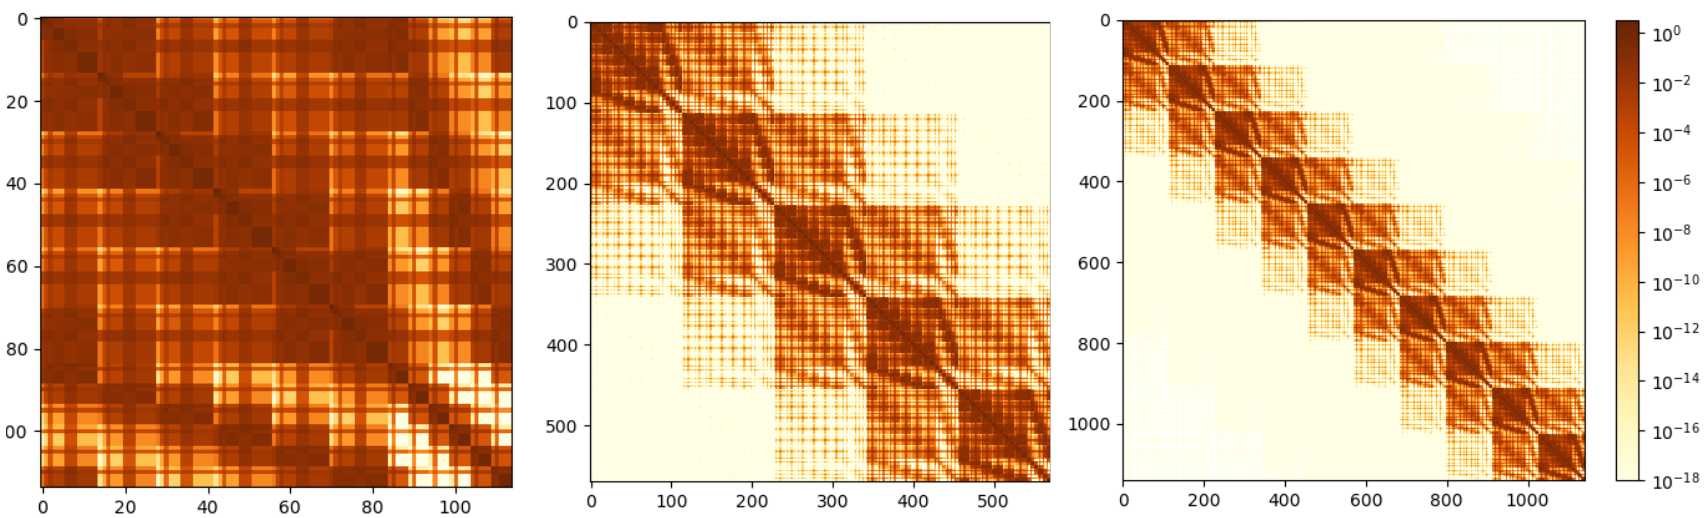
\includegraphics[scale=0.2]{figures/sparsity_plots/sparsity_masks.png} \caption{Schwarz sparsity masks used for benzene stacks containing 
1, 5, and 10 benzenes spaced 3\text{\AA}  apart. Sparsity masks were obtained by evaluating $(\mu\nu|\mu\nu)<\frac{\tau^2}{(\mu\nu|\mu\nu)_{max}}$.}
\label{fig:databases} \end{figure}


\section{Integral Construction}

Now, we are equipped to discuss the resulting algorithms when applying the integral sparsity to important operations such as
integral construction and transformation. To write more readable algorithms, 
we employ some tensor notation and write $A_{\mu \nu}^P$ to represent
the pre-contracted 3-center integrals $(\mu \nu |P)$. To prune these integrals using sparsity, 
the following algorithm can be employed:

\begin{algorithm}
\caption{Prune $A_{\mu \nu}^P$ using sparsity}
\begin{algorithmic}
\REQUIRE AO integrals: $A_{\mu \nu}^P$, screening mask: $S_{\mu \nu}^b$
\FOR {$\mu = 0$ to $\mu = N_{AO}-1$}  
    \STATE $A_{\mu \nu}^P S_{\mu \nu}^b \rightarrow A_{\mu \nu^{\mu}}^P$
\ENDFOR
\RETURN $A_{\mu \nu^\mu}^P$
\end{algorithmic}
\end{algorithm}

\noindent Here we have introduced the symbol $\nu^\mu$, which indicates that $\nu$ is restricted to AO functions
which are spatially close enough to $\mu$ to survive the Schwarz screening process. The superscript in $\nu^\mu$ 
indicates a dependence of $\nu$ according to $\mu$. Algorithm 1 is purely pedagogical, as one would never
build the full $A_{\mu \nu}^P$ integrals and then prune them for sparsity. 
Rather, sparsity screening would be applied as the integrals are constructed and insignificant
function triplets are never computed. The computation
and storage of $A_{\mu \nu^\mu}^P$ scales as $\mathcal{O}(N_{aux}N_{AO}^{1-2})$. 
Moreover, the costly metric contraction becomes
\begin{align} 
B_{\mu \nu^\mu}^Q = A_{\mu \nu^\mu}^P[J]_{PQ}^{-\frac{1}{2}}
\end{align}
\noindent and scales as $\mathcal{O}(N_{aux}^2N_{AO}^{1-2})$, where the lower bound is achieved for sufficiently sparse
systems.

\section{Integral Transformation}

The transformation of $A_{\mu \nu}^P$ (or $B_{\mu \nu^\nu}^Q$) from the AO basis to the MO basis is 
an essential operation for many quantum 
chemistry procedures. The operation requires two MO matrices: $C_{\mu p}, C_{\nu q}$, where $p, q$ are MO space
indices. These matrices will be identical if $p$ and $q$ run over the full space of MOs, but could be different if $p$ and $q$
belong to two different subsets of MOs (e.g., occupied orbitals and unoccupied orbitals).
A first contraction $A_{p \nu}^P=A_{\mu \nu}^PC_{\mu p}$ will half-transform the integrals and costs 
$\mathcal{O}(N_{aux}N_{AO}^2N_p)$. The second contraction $A_{p q}^P=A_{p \nu}^PC_{\nu q}$ will cost
$\mathcal{O}(N_{aux}N_{AO}N_pN_q)$.
Note the first contraction should involve the smaller of $N_p$ and $N_q$ in order to reduce complexity. Also, the first contraction
is comparably more expensive than the latter since the size of the AO space is larger than any MO space. Therefore,
reducing the cost of the first contraction would alleviate a bottleneck overall. 
Thankfully, we can exploit the sparsity of $A_{\mu \nu^\mu}^P$.
To do so, we carry out a looping DGEMM through the $\mu$ index and apply the sparsity mask to the orbital matrix $C_{\mu p}$.
Algorithm 2 illustrates the resulting process:

\begin{algorithm}[H]
\caption{Transform sparse integrals $A_{\mu \nu^\mu}^P$ to MO spaces.}
\begin{algorithmic}
\REQUIRE Sparse AO integrals: $A_{\mu \nu^\mu}^P$, orbital matrices: $C_{\mu p}, C_{\nu q}$, screening mask: $S_{\mu \nu}^b$
\FOR {$\mu = 0$ to $\mu = N_{AO}-1$}  
    \STATE $C_{\nu q}S_{\mu \nu}^b \rightarrow C_{\nu^{\mu} q}$
    \STATE $A_{\mu \nu^{\mu}}^P C_{\nu^{\mu} q} \rightarrow A_{\mu q}^P$
\ENDFOR
\STATE $A_{\mu q}^PC_{\mu p} \rightarrow A_{p q}$
\RETURN $A_{p q}^P$
\end{algorithmic}
\end{algorithm}


\section{Results}

All methods were implemented in the {\sc Psi4} electronic structure software package \cite{Parrish:2017:3185}.
The parallelism in {\sc Psi4} relies on the shared memory programming model using OpenMP 
and carries out matrix multiplications using Intel's Math Kernel
Library. 

We demonstrate the performance of our Schwarz screening implementation 
by measuring the performance when computing the 3-center integrals, contracting the fitting metric,
and transforming the integrals into an MO basis.
The experiment employed an ideal sparse system: stacked benzenes. Execution times were recorded for each successive benzene
added to the stack, from one to ten benzenes, with each benzene spaced 5\AA\ apart.
Transformation time involved the wall time required to carry out the common occupied-virtual
transformation, as would be required by density-fitted MP2: 
\begin{align} 
(i b | Q) = (\lambda \sigma | Q) C_{\sigma i} C_{\lambda b} 
\end{align}

\noindent Where $i, j$ and $a, b$ denote occupied and virtual spaces, respectively. 
Algorithm 2 was implemented and used to carry out these transformations.
The cc-pVTZ and cc-pVTZ-jkfit basis sets were used for primary 
and auxiliary basis sets, respectively. The characteristics
of each system are listed in Table 2.1. The mask sparsity listed in Table 2.1 refers to the percentage of non-significant AO function pairs appearing in the sparsity mask.
The experiment was carried out using one node consisting of an Intel Core i7-5930K processor 
(6 cores at 3.50GHz) and 50GB DRAM. The results are plotted in Figure 2.2. Figure 2.2 (a), (b), (c), and (d) involve time to compute the 3-index integrals, contract the fitting metric,
perform the first transformation step: $(\mu \nu | Q)C_{i \mu} \rightarrow (i \nu | Q)$,
and total transform time, respectively.
Note that our novel contribution involves the application of the sparsity screening in the transformation step.

\begingroup
\begin{table}[H]
\centering
\renewcommand{\baselinestretch}{1}
\caption{Characteristics of benzene stack systems. $N$ and $N_{aux}$ refer to the number of primary and auxiliary basis functions, respectively.
 Mask sparsity refers to the percentage of significant AO function pairs in the sparsity mask. Mask sparsity increases with additional benzenes added to the stack.}
\begin{tabular}{l ccc}
\multicolumn{1}{l}{\textbf{Benzenes}} &
\multicolumn{1}{c}{\textbf{$N$}} &
\multicolumn{1}{c}{\textbf{$N_{aux}$}} &
\multicolumn{1}{c}{\textbf{Mask Sparsity (\%)}} \\
\hline
1        & 264  & 654       & 2.6              \\ 
2        & 528  & 1308      & 24.7             \\ 
3        & 792  & 1962      & 43.6             \\ 
4        & 1056 & 2616      & 55.3             \\ 
5        & 1320 & 3270      & 63.1             \\ 
6        & 1584 & 3924      & 68.6             \\ 
7        & 1848 & 4578      & 72.7             \\ 
8        & 2112 & 5232      & 75.9             \\ 
9        & 2376 & 5886      & 78.4             \\ 
10       & 2640 & 6540      & 80.4             \\ 
\end{tabular}
\end{table}
\endgroup

\begin{figure}[H]
  \centering
  \subfloat[]{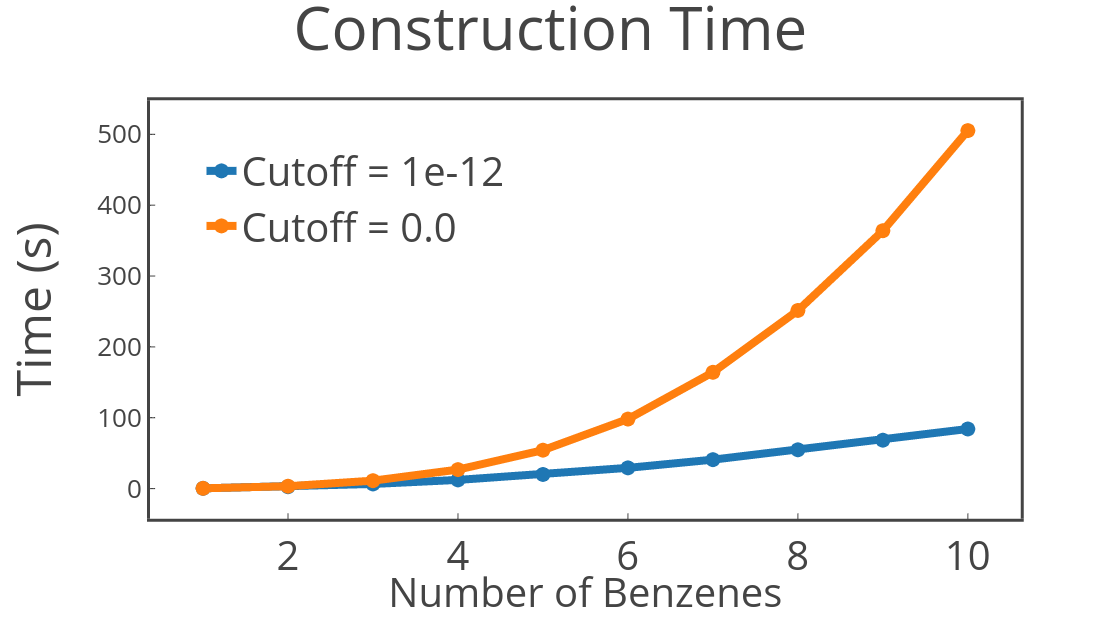
\includegraphics[width=0.5\textwidth]{figures/sparsity_plots/construction_wall.png}\label{fig:f1}}
  \hfill
  \subfloat[]{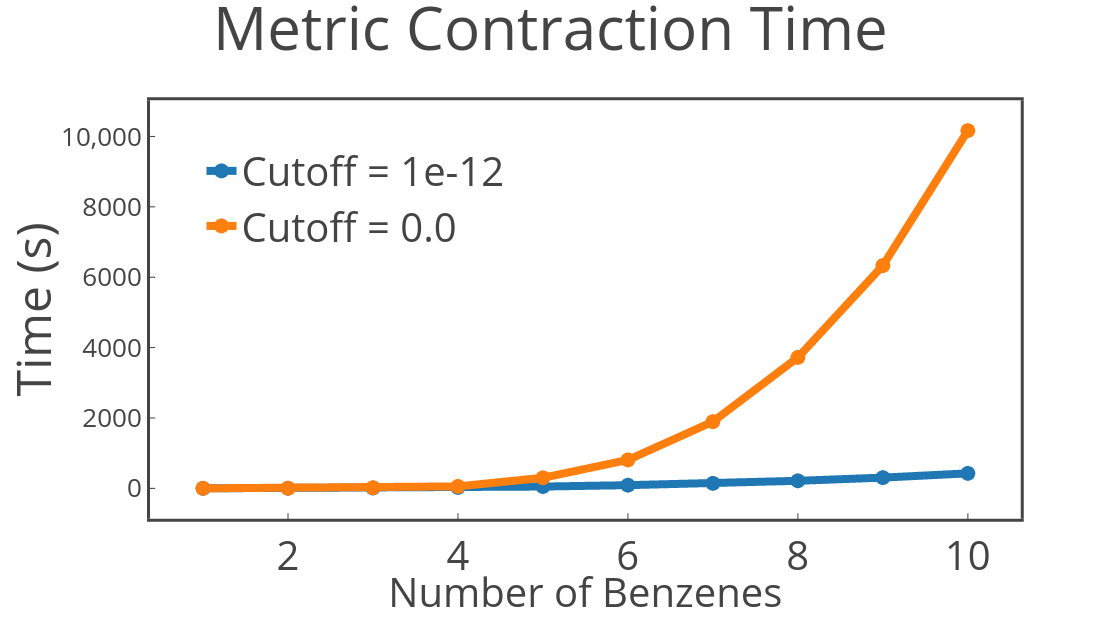
\includegraphics[width=0.5\textwidth]{figures/sparsity_plots/metric_contraction.png}\label{fig:f1}}
  \hfill \\
  \subfloat[]{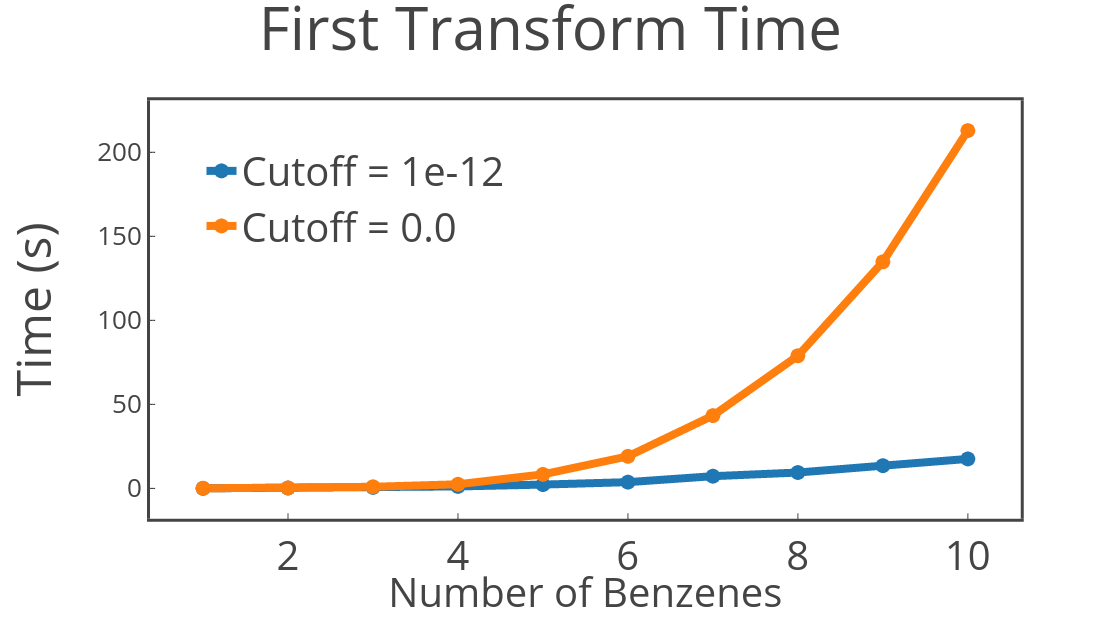
\includegraphics[width=0.5\textwidth]{figures/sparsity_plots/first_transform_wall.png}\label{fig:f1}}
  \hfill
  \subfloat[]{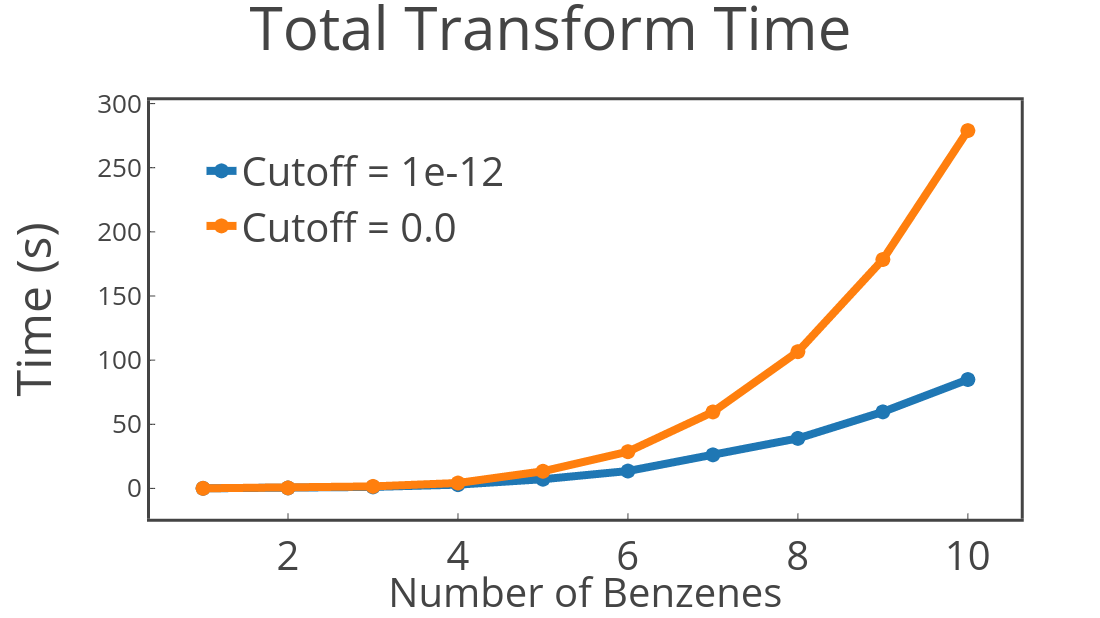
\includegraphics[width=0.5\textwidth]{figures/sparsity_plots/total_transform_wall.png}\label{fig:f2}}
  \caption{Comparison of execution times using sparsity screening (blue) against no sparsity screening (orange). Execution time is plotted against number of benzenes
 in a benzene stack from one to ten benzenes. Transformations involved computing $(ib|Q)$, where $i$ and $b$ denote occupied and virtual indices, respectively.
 Cutoff refers to the Schwarz screening threshold. (a) Computing the integrals. (b) Contracting AO integrals with the fitting metric. 
(c) First transformation times only. (d) Sum of first and second transformation times.}
\end{figure}

\noindent The cost of the first contraction becomes $\mathcal{O}(N_{aux}N_{AO}^{1-2}N_p)$. 
The remaining sparsity in the half-transformed $A_{\nu q}^P$ is unrelated to the original sparsity mask.

\begingroup
\begin{table}[H]
\centering
\renewcommand{\baselinestretch}{1}
\caption{Speedups obtained from sparsity screening at ten benzenes from data in Figure 2.2.}
\begin{tabular}{l c}
\multicolumn{1}{l}{\textbf{Operation}} &
\multicolumn{1}{c}{\textbf{Speedup at 10 benzenes}} \\ 
\hline
Construction          & 10.6  \\          
Metric Contraction    & 37.8  \\          
First Transformation  & 25.8  \\          
Total Transformation  & 5.5  \\          
\end{tabular}
\end{table}
\endgroup


Clearly, Figure 2.2 reveals significant time reductions for all procedures measured.
Table 2.2 reinforces that operations with higher complexity scaling have the largest time
reduction, with the caveat that total transformation time includes portions without sparsity utilization.
In the integral computations (Figure 2.2 (a)), we construct the sparse integrals using
function screening; however, we still compute them in shells for efficiency.
Therefore the acquired speedup is slightly less dramatic compared to the metric contraction and
transformation procedures (Figure 2.2 (b) and (c), respectively) due to select functions being 
screened in cases where the entire shell is not screened. 
Note that the metric contraction is by far the most expensive operation, which should in one part
highlight the boon of sparsity utilization and in another part
illustrate the pertinence of our workflow investigation in Chapter 3 of this thesis.
Last, our proposal outlined in Algorithm 2 for applying sparsity screening to integral transformations
is proven viable by Figure 2.2 (c). Note that significant reductions are obtained for the
first transformation; however, the sparsity mask constructed is not helpful for the second transformation step.
With sparsity utilization, the first step scales as $\mathcal{O}(N_{aux}N_{AO}^{1-2}p)$,
whereas the second transformation step will still scale as $\mathcal{O}(N_{aux}N_pN_q)$.
In this work we have not gone on to consider sparsity of the MO indices, which would 
typically require transformation to local orbitals.




%%%%%%%%%%%%%%%%
% Chapter 3
%%%%%%%%%%%%%%%%

\chapter{Optimizing Integral Transformations}

\section{A note on disk-bound blocking}

The size of tensors grow rapidly in quantum chemistry.  The 3-center integrals of density fitting are no exception.
Often, as the size of the AO three-index integrals will exceed 50GB of RAM for systems as small as 40 atoms when
a moderate basis set such as aug-cc-pVQZ is used, even with sparsity screening.  At that point, it is necessary for
any implementation to begin reading and writing these tensors to and from disk-based memory. For any field this can
be a major slowdown, but it is especially critical for performance when high dimensional data is involved. To illustrate
this issue, I will introduce an adapted tensor notation which better indicates memory layout.

We denote an $n$-dimensional tensor as $T_{ab\hdots n}$, where the indices from left to right go from the slowest-running
to the fastest-running indices. Here, $a$ is the slowest-running index, $b$ is the next slowest-running
index, and $n$ is the fastest-running index. The choice of memory layout plays a crucial role when indices are being accessed.
Iterating through the slowest-running index, $a$, would require the largest memory strides whereas the elements 
of the fastest-running index, $n$, are contiguous in memory. 

Now, we can consider two possible forms for the 3-index integrals: $A_{P\mu\nu}$ or $A_{\mu P\mu}$.
If these tensors are too large to fit into memory, we must read and write pieces of them to and from disk-based memory.
To accomplish this, we must choose an index to block accross. Primarily, this will involve either the $P$ or $\mu$ index.
For example, if we choose to block accross the $P$ index, then we will partition the basis of $P$ into discrete blocks:
\begin{align}
a;lkds
\end{align}

Then, we will read and write only those blocks of $P$ along with all of $\mu$ and $\nu$. The latency of these operations is
bound by the movement of a physical read-write head, so it is critically important to ensure that read and writes are as
contiguous as possible. In the case of $P$ blocking, the $A_{P\mu\nu}$ tensor is far superior to $A_{\mu P\mu}$ since the 
former will yield entirely contiguous operations whereas the latter will require strided operations.  








%%%%%%%%%%%%%%%%
% Chapter 4
%%%%%%%%%%%%%%%%

\chapter{Evaluating Coulomb and Exchange Matrices}

\section{Coulomb and Exchange Evaluations}

From Chapter 1, we wrote the most efficient evaluations of the three-index ERIs to build the Coulomb and exchange matrices as:

\begin{align}
J_{\mu \nu} &= B_{\mu \nu}^P B_{\lambda \sigma}^PD_{\lambda \sigma} \\
K_{\mu \nu} &= B_{\mu \lambda}^P B_{\nu \sigma}C_{p\lambda}C_{p\sigma},
\end{align}

\noindent where (4.1) and (4.2) are evaluated in $\mathcal{O}(N_{AO}^2N_{aux})$ and $\mathcal{O}(N_{AO}^2N_{aux}N_p)$ operations, respectively.
The exchange matrix evaluation is a major bottleneck within the density fitting regime. The focus of this chapter is on analyzing and improving
exchange builds to take advantage of sparsity, optimize parallel scaling, and to minimize disk operations.
Thankfully, it turns out that Algorithm 6 is easily 
extendible to (4.2). In fact, if one uses orbital matrices to build the exchange matrix as in (4.2), the half-transformed 
intermediate generated during integral transformations, $B_{\mu Pq}$, is actually identical to the intermediate when building the exchange matrix. 
Moreover, the memory layout of $B_{\mu Pq}$ is ideal for the subsequent contraction to form $K$. The following algorithm results:

\begin{algorithm}[H]
\caption{Building the $K$ matrix.}
\begin{algorithmic}
\REQUIRE Sparse AO integrals: $B_{\mu P \nu^\mu}$, orbital matrices: $C_{\mu p}, C_{\nu p}$, screening mask: $S_{\mu \nu}^b$
\FOR {$\mu = 0$ to $\mu = N_{AO}-1$}  
    \STATE Trim from dense to sparse: $C_{\nu p}S_{\mu \nu}^b \rightarrow C_{\nu^{\mu} p}$
    \STATE $B_{\mu P \nu^{\mu}} C_{\nu^{\mu} p} \rightarrow T_{\mu Pp}$
    \IF {$C_{\mu p} != C_{\nu p}$}
        \STATE Trim from dense to sparse: $C_{\mu p}S_{\mu \nu}^b \rightarrow C_{\mu^{\nu} p}$
        \STATE $B_{\nu P \mu^{\nu}} C_{\mu^{\nu} p} \rightarrow T_{\nu P p}$
    \ELSE
        \STATE $T_{\nu P p} = T_{\mu P p}$ 
    \ENDIF
\ENDFOR
\STATE $T_{\mu P q} T_{\nu P q} \rightarrow K_{\mu \nu} $
\RETURN $K_{\mu \nu}$
\end{algorithmic}
\end{algorithm}

We have used $T$ tensors to indicate intermediates.
Algorithm 9 is an ideal candidate for building the $K$ matrix, as it both utilizes sparsity and maximizes concurrency.
However, while it may be assumed that both $J$ and $K$ can always fit within in-core memory constraints, the same is not true 
for the three-index AO integrals. Therefore, we must consider the behavior of Algorithm 9 when the 
in-core memory is constrained such that it becomes necessary to perform blocking operations accross the $P$ index. Then, the algorithm
becomes: 

\begin{algorithm}[H]
\caption{Building the $K$ matrix using $B_{\mu P \nu^\mu}$, blocking accross $P$}
\begin{algorithmic}
\REQUIRE Sparse AO integrals: $B_{\mu P \nu^\mu}$, orbital matrices: $C_{\mu p}, C_{\nu p}$, screening mask: $S_{\mu \nu}^b$
\FOR {block $P_i \in P$}    
    \STATE Read from disk: $B_{\mu P_i \nu^{\mu}}$
    \FOR {$\mu = 0$ to $\mu = N_{AO}-1$}  
        \STATE Trim from dense to sparse: $C_{\nu p}S_{\mu \nu}^b \rightarrow C_{\nu^{\mu} p}$
        \STATE $B_{\mu P_i \nu^{\mu}} C_{\nu^{\mu} p} \rightarrow T_{\mu P_i p}$
        \IF {$C_{\mu p} != C_{\nu p}$}
            \STATE Trim from dense to sparse: $C_{\mu p}S_{\mu \nu}^b \rightarrow C_{\mu^{\nu} p}$
            \STATE $B_{\nu P_i \mu^{\nu}} C_{\mu^{\nu} p} \rightarrow T_{\nu P_i p}$
        \ELSE
            \STATE $T_{\nu P_i p} = T_{\mu P_i p}$ 
        \ENDIF
    \ENDFOR
    \STATE $K_{\mu \nu} = K_{\mu \nu} + T_{\mu P_i q} T_{\nu P_i q}$
\ENDFOR
\RETURN $K_{\mu \nu}$
\end{algorithmic}
\end{algorithm}

\noindent Unfortunately, this algorithm will require strided disk operations when reading the $B_{\mu P^i \nu^{\mu}}$ tensor into memory.
Since poor disk IO can drastically decrease performance, it is often better to force disk operations 
to be contiguous and transpose any tensors as necessary in core memory. Since it is best to block accross the $P$ index (as discussed in
Chapter 3), a better
memory layout for the sparse integrals is the $B_{P \mu \nu^\mu}$ form, since this form will allow for completely 
contiguous reads from disk memory. Another possible algorithm can then be formualted:

\begin{algorithm}[H]
\caption{Building the $K$ matrix using $B_{P \mu \nu^\mu}$, blocking accross $P$}
\begin{algorithmic}
\REQUIRE Sparse AO integrals: $B_{P \mu \nu^\mu}$, orbital matrices: $C_{\mu p}, C_{\nu p}$, screening mask: $S_{\mu \nu}^b$
\FOR {block $P_i \in P$}
    \STATE Read from disk: $B_{P_i \mu \nu^{\mu}}$
    \FOR {$\mu = 0$ to $\mu = N_{AO}-1$}  
        \STATE Copy: $B_{P_i \mu \nu^{\mu}} \rightarrow b_{P_i \nu^{\mu}}$
        \STATE Trim from dense to sparse: $C_{\nu p}S_{\mu \nu}^b \rightarrow C_{\nu^{\mu} p}$
        \STATE $b_{P_i \nu^{\mu}} C_{\nu^{\mu} p} \rightarrow T_{\mu P_i p}$
        \IF {$C_{\mu p} != C_{\nu p}$}
            \STATE Trim from dense to sparse: $C_{\mu p}S_{\mu \nu}^b \rightarrow C_{\mu^{\nu} p}$
            \STATE $b_{P_i \mu^{\nu}} C_{\mu^{\nu} p} \rightarrow T_{\nu P_i p}$
        \ELSE
            \STATE $T_{\nu P_i p} = T_{\mu P_i p}$ 
        \ENDIF
    \ENDFOR
    \STATE $K = K +  T_{\mu P_i p} T_{\mu P_i p} $
\ENDFOR
\RETURN $K$
\end{algorithmic}
\end{algorithm}

\noindent Here, we used a buffer, $b_{P^i \nu^{\mu}}$, to transpose pieces of $B_{P^i \mu \nu^{\mu}}$ while looping over $\mu$.
Although this algorithm may involve a strided copy and additional memory usage, the disk reads for the $B_{P^i \mu \nu^{\mu}}$ 
tensor are completely contiguous. 
For smaller investigations, the three-index AO integrals can be fit completely in-core and Algorithm 10 should yield superior 
performance. However, for larger systems,
the strided disk reads in Algorithm 10 may cause performance degredation to the point that Algorithm 11 will become superior.

Although the exchange matrix evaluation is the primary computational bottleneck, it is important to note how the above integral
formats will affect Coulomb matrix evaluations. To build the Coulomb matrix, the sparsity mask can be applied
directly to the density matrix. The following algorithm results:

\begin{algorithm}[H]
\caption{Building the $J$ matrix.}
\begin{algorithmic}
\REQUIRE Sparse AO integrals: $B_{\mu \nu^{\mu}}^P$, density matrix: $D_{\mu \nu}$, screening mask: $S_{\mu \nu}^b$
\STATE Trim from dense to sparse: $D_{\mu \nu}S_{\mu \nu}^b \rightarrow D_{\mu \nu^{\mu} }$
\STATE $B^P_{\mu\nu^{\mu}} D_{\mu \nu^{\mu}} \rightarrow T^{P}$
\STATE $T^{P} B^P_{\mu \nu^{\mu}} \rightarrow J_{\mu \nu^{\mu}} $
\STATE Unpack from sparse to dense: $J_{\mu \nu^{\mu}} \rightarrow J_{\mu \nu}$
\RETURN $J_{\mu \nu}$
\end{algorithmic}
\end{algorithm}

\noindent Moreover, the corresponding disk-based implementations for the $B_{\mu P \nu^\mu}$ and $B_{P \mu \nu^\mu}$ integral
formats are listed in Algorithms 13 and 14, respectively.

\begin{algorithm}[H]
\caption{Building the $J$ matrix using $B_{\mu P \nu^\mu}$, blocking accross $P$}
\begin{algorithmic}
\REQUIRE Sparse AO integrals: $B_{\mu P \nu^{\mu}}$, density matrix: $D_{\mu \nu}$, screening mask: $S_{\mu \nu}^b$
\FOR {block $P_i \in P$}
    \STATE Read from disk: $B_{\mu P_i \nu^{\mu}}$
    \STATE Initialize: $T_{P_i} = 0$
    \FOR {$\mu = 0$ to $\mu = N_{AO}-1$}  
        \STATE Copy to sparse: $D_{\mu \nu}S_{\mu \nu}^b \rightarrow d_{\nu^{\mu} }$
        \STATE $T_{P_i} = T_{P_i} + B_{\mu P_i \nu^{\mu}}d_{\nu^{\mu}}$
    \ENDFOR    
    \STATE $T_{P_i} B_{P_i \mu \nu^{\mu}} \rightarrow J_{\mu \nu^{\mu}} $
    \STATE Unpack from sparse to dense: $J_{\mu \nu^{\mu}} \rightarrow J_{\mu \nu}^{\{P_i\}}$
    \STATE $J_{\mu \nu} = J_{\mu \nu} + J_{\mu \nu}^{\{P_i\}}$
\ENDFOR
\RETURN $J_{\mu \nu}$
\end{algorithmic}
\end{algorithm}

\begin{algorithm}[H]
\caption{Building the $J$ matrix using $B_{P \mu \nu^\mu}$, blocking accross $P$}
\begin{algorithmic}
\REQUIRE Sparse AO integrals: $B_{P \mu \nu^{\mu}}$, density matrix: $D_{\mu \nu}$, screening mask: $S_{\mu \nu}^b$
\FOR {block $P_i \in P$}
    \STATE Read from disk: $B_{P_i \mu \nu^{\mu}}$
    \STATE Trim from dense to sparse: $D_{\mu \nu}S_{\mu \nu}^b \rightarrow D_{\mu \nu^{\mu} }$
    \STATE $B_{P_i \mu\nu^{\mu}} D_{\mu \nu^{\mu}} \rightarrow T^{P_i}$
    \STATE $T^{P_i} B_{P_i \mu \nu^{\mu}} \rightarrow J_{\mu \nu^{\mu}} $
    \STATE Unpack from sparse to dense: $J_{\mu \nu^{\mu}} \rightarrow J_{\mu \nu}^{\{P_i\}}$
    \STATE $J_{\mu \nu} = J_{\mu \nu} + J_{\mu \nu}^{\{P_i\}}$
\ENDFOR
\RETURN $J_{\mu \nu}$
\end{algorithmic}
\end{algorithm}

\noindent Here, we have used the superscript in $J_{\mu \nu}^{\{P_i\}}$ to indicate the contribution to 
$J_{\mu \nu}$ corresponding to the $P_i$ block.
Note that Algorithm 13 is likely inferior to Algorithm 14, with both necessary loops and copies as well as non-contiguous disk reads.
However, since Coulomb matrix evaluation requires considerably less compute time than the exchange matrix evaluations, 
the performance of Algorithms 13 and 14 will be nearly trivial. Moreover, note that the disk reads in Algorithms 10 and 13 as well as 
in Algorithms 11 and 14 will be occuring simulataneously. The $J$ and $K$ computational kernel will generally take this form:

\begin{algorithm}[H]
\caption{Coulomb and exchange matrix evaluation kernel.}
\begin{algorithmic}
\REQUIRE Sparse AO integrals: $B^P_{\mu \nu^{\mu}}$, density matrix: $D_{\mu \nu}$, orbital matrices: $C_{\mu p}, C_{\nu p}$, screening mask: $S_{\mu \nu}^b$
\STATE Initialize temps.
\FOR {block $P_i \in P$}
    \STATE Read from disk: $B^{P_i}_{\mu \nu^{\mu}}$
    \STATE J = ComputeJ($B^{P_i}_{\mu \nu^{\mu}}$, $S_{\mu \nu}^b$, $D_{\mu \nu}$)
    \STATE K = ComputeK($B^{P_i}_{\mu \nu^{\mu}}$, $S_{\mu \nu}^b$, $C_{\mu p}, C_{\nu p}$)
\ENDFOR
\RETURN $J_{\mu \nu}$, $K_{\mu \nu}$
\end{algorithmic}
\end{algorithm}

\noindent An implementation of this kernel will involve using the $B_{\mu P \nu^\mu}$ integral form with Algorithms 10 and 13 or the 
$B_{\mu P \nu^\mu}$ integral form with Algorithms 11 and 14. In the next section, we discuss the performance of these choices in practice.

\section{Results}

All methods were implemented in the {\sc Psi4} electronic structure software package.
The parallelism in {\sc Psi4} relies on the shared memory programming model using OpenMP 
and carries out matrix multiplications using Intel's Math Kernel
Library. Currently, the state of the art for exchange matrix evaluations in
{\sc Psi4} is Algorithm 11. However, we conjecture that Algorithm 10 could provide 
considerable speedups as it eliminates entirely a strided, level 1 BLAS copy. 

We implemented Algorithms 10 and 13 and incorporated them into a development version of {\sc Psi4}. 
Then, we used {\sc Psi4}'s Self-Consistent Field
procedure to produce energies for various systems and basis set combinations. The systems used involved a protein-drug complex,
where the drug molecule is ommitted and the atoms of the protien are added in a series according to distance from the center of
the drug molecule. 

The experiments were carried out using one node consisting of an Intel Core i7-5930K processor
(6 cores at 3.50GHz) and 60GB DRAM. The results are included in Table 4.1:

\begingroup
%\squeezetable
\renewcommand{\arraystretch}{0.7}
\begin{table}[H]
\footnotesize
\centering
\renewcommand{\baselinestretch}{1}
\caption{Total execution times for SCF procedures accross various systems using Algorithms 10 and 11 for exchange matrix evaluations. 
The corresponding Coulomb matrix evaluations were performed using Algorithms 13 and 14, respectively. Total wall times include 
wall time for the entire program to execute. J and K compute time indicates the total time spent in the Coulomb and exchange matrix
evaluation kernels, respectively. System descriptions including number of AO basis functions, $N_{AO}$, number of auxiliary basis functions,
$N_{aux}$, basis, and number of atoms, $N_{at.}$, are included in the leftmost columns. All rows are sorted by the product: $N_{aux}N_{AO}$.
A speedup column is included for total wall time and is calculated as the total prcedure time spent using Algorithms 11 and 14 dived by 
the total procedure time spent using Algorithms 10 and 13.
\label{tbl:practical_speedups}}
\begin{tabular}{lrrrrrrrrrr}
  \multicolumn{1}{c}{\textbf{}} 
& \multicolumn{1}{c}{\textbf{}} 
& \multicolumn{1}{c}{\textbf{}} 
& \multicolumn{1}{c}{\textbf{}} 
& \multicolumn{3}{c}{\textbf{Total Wall Time}}  
& \multicolumn{2}{c}{\textbf{J Compute Time}}  
& \multicolumn{2}{c}{\textbf{K Compute Time}} \\ 
\cline{5-7}
\cline{8-9}
\cline{10-11}
  \multicolumn{1}{c}{\textbf{$N_{AO}$}} 
& \multicolumn{1}{c}{\textbf{$N_{aux}$}} 
& \multicolumn{1}{c}{\textbf{Basis}} 
& \multicolumn{1}{c}{\textbf{$N_{at.}$}} 
& \multicolumn{1}{c}{\textbf{10 \& 13}} 
& \multicolumn{1}{c}{\textbf{11 \& 14}} 
& \multicolumn{1}{c}{\textbf{spdup}} 
& \multicolumn{1}{c}{\textbf{Alg. 10}} 
& \multicolumn{1}{c}{\textbf{Alg. 11}} 
& \multicolumn{1}{c}{\textbf{Alg. 13}} 
& \multicolumn{1}{c}{\textbf{Alg. 14}} \\ 
\hline
 147&  721&    DZ&    15&                 3.8 &                4.7&     1.2 &                0.1 &                0.0&                 0.5&                 0.6\\
 247&  912&   aDZ&    15&                 5.8 &                7.7&     1.3 &                0.2 &                0.1&                 1.4&                 2.1\\
 338&  842&    TZ&    15&                 7.5 &                9.9&     1.3 &                0.2 &                0.2&                 2.3&                 3.3\\
 294& 1442&    DZ&    30&                12.4 &               18.1&     1.5 &                0.3 &                0.3&                 5.6&                 7.1\\
 529& 1154&   aTZ&    15&                18.7 &               29.9&     1.6 &                0.8 &                0.8&                 7.4&                13.1\\
 375& 1837&    DZ&    39&                25.4 &               36.8&     1.4 &                0.5 &                0.5&                13.3&                16.6\\
 650& 1205&    QZ&    15&                24.7 &               43.8&     1.8 &                1.2 &                1.1&                11.1&                19.3\\
 494& 1824&   aDZ&    30&                35.3 &               54.8&     1.6 &                1.0 &                0.9&                18.1&                25.7\\
 676& 1684&    TZ&    30&                46.0 &               74.7&     1.6 &                1.2 &                1.2&                28.2&                38.6\\
 522& 2558&    DZ&    54&                72.3 &              109.2&     1.5 &                1.1 &                0.9&                48.8&                56.8\\
 631& 2328&   aDZ&    39&                81.5 &              132.9&     1.6 &                2.1 &                2.0&                46.8&                65.1\\
 603& 2953&    DZ&    63&               117.2 &              166.9&     1.4 &                1.3 &                1.1&                83.2&                92.4\\
 866& 2150&    TZ&    39&               109.3 &              176.6&     1.6 &                2.5 &                2.4&                74.7&                97.6\\
1058& 2308&   aTZ&    30&               145.5 &              278.9&     1.9 &                4.6 &                4.7&                91.0&               138.6\\
 756& 3696&    DZ&    81&               231.3 &              328.3&     1.4 &                1.8 &                1.6&               176.3&               190.9\\
 878& 3240&   aDZ&    54&               232.0 &              394.4&     1.7 &                4.6 &                4.4&               161.9&               206.3\\
1300& 2410&    QZ&    30&               218.0 &              376.1&     1.7 &                5.6 &                5.8&               148.7&               198.3\\
1204& 2992&    TZ&    54&               332.5 &              504.1&     1.5 &                4.9 &                4.7&               256.8&               302.4\\
1015& 3744&   aDZ&    63&               403.1 &              640.8&     1.6 &                6.3 &                6.1&               305.2&               361.9\\
1357& 2954&   aTZ&    39&               385.9 &              726.9&     1.9 &               10.5 &               12.3&               259.2&               376.6\\
 974& 4766&    DZ&   103&               629.3 &              845.3&     1.3 &                3.6 &                3.2&               520.0&               549.7\\
1394& 3458&    TZ&    63&               601.7 &              850.5&     1.4 &                6.6 &                6.2&               492.8&               551.2\\
1670& 3089&    QZ&    39&  1153.5$^{\dagger}$ &              933.4&     0.8 &   12.8$^{\dagger}$ &               13.2&   395.5$^{\dagger}$&               504.7\\
1275& 4698&   aDZ&    81&               898.9 &             1379.0&     1.5 &               10.6 &               10.7&               711.5&               813.2\\
1758& 4341&    TZ&    81&              1372.3 &             1839.0&     1.3 &               10.2 &                9.8&              1176.8&              1269.1\\
1886& 4108&   aTZ&    54&  3811.0$^{\dagger}$ &             2164.0&     0.6 &   25.8$^{\dagger}$ &               26.2&   931.2$^{\dagger}$&              1183.4\\
1641& 6050&   aDZ&   103&  4406.9$^{\dagger}$ &             3528.3&     0.8 &   23.9$^{\dagger}$ &               24.6&  1958.4$^{\dagger}$&              2161.9\\
2320& 4294&    QZ&    54&  4280.4$^{\dagger}$ &             2741.3&     0.6 &   26.3$^{\dagger}$ &               25.0&  1377.2$^{\dagger}$&              1611.1\\
2185& 4754&   aTZ&    63&  5744.9$^{\dagger}$ & 4594.0$^{\dagger}$&     0.8 &   37.3$^{\dagger}$ &   37.0$^{\dagger}$&  1727.3$^{\dagger}$&  2063.1$^{\dagger}$\\
2258& 5589&    TZ&   103&  5474.8$^{\dagger}$ &             4710.6&     0.9 &   23.5$^{\dagger}$ &               20.2&  3228.0$^{\dagger}$&              3381.7\\
2690& 4973&    QZ&    63&  6892.9$^{\dagger}$ &             4581.9&     0.7 &   39.5$^{\dagger}$ &               33.7&  2598.4$^{\dagger}$&              2893.4\\
2760& 5988&   aTZ&    81& 11294.6$^{\dagger}$ & 9350.0$^{\dagger}$&     0.8 &   64.6$^{\dagger}$ &   63.4$^{\dagger}$&  4003.6$^{\dagger}$&  4669.9$^{\dagger}$\\
3405& 6276&    QZ&    81& 14075.7$^{\dagger}$ &11354.3$^{\dagger}$&     0.8 &   70.6$^{\dagger}$ &   54.7$^{\dagger}$&  6318.9$^{\dagger}$&  6829.2$^{\dagger}$\\
3542& 7696&   aTZ&   103& 28136.3$^{\dagger}$ &23132.6$^{\dagger}$&     0.8 &  144.4$^{\dagger}$ &  124.7$^{\dagger}$& 11201.2$^{\dagger}$& 12464.4$^{\dagger}$\\

\hline
\end{tabular}
\renewcommand{\thefootnote}{\fnsymbol{footnote}}
\footnote[2]{} Indicates a disk-based implementation was used.
\end{table}
\endgroup

Note that the $^{\dagger}$ symbol is used to indicate when a disk-based implementation is required. For Algorithm 11, it is possible
to store up to half of the AO function pairs by applying permuatational symmetry. The necessary copy, 
$B_{P_i \mu \nu^{\mu}} \rightarrow b_{P_i \nu^{\mu}}$, allows for this. Doing so effectively halves the memory requirement for Algorithm 11
with respect to Algorithm 10. For this reason, Algorithm 10 is forced to resort to a disk-based implementation sooner than Algorithm 11.

The results in Table 4.1 confirms our analysis of Algorithms 10 and 11. For small enough investigations, Algorithm 10 will always be more
efficient. Total time spent in the exchange matrix evaluation kernel is always smaller for Algorithm 10. Only when Algorithm 10 switches to 
a disk-based implementation that requires strided disk reads does it become slower than Algorithm 11 overall. Moreover, since the scaling of
the Coulomb matrix evaluation is an entire factor smaller than the exchange matrix evaluation, its required time is almost trivial overall.

Last, note that the total time spent in the $J$ and $K$ evaluations does not entirely account for the differences in performance. The 
remaining difference involves the computation of $B^P_{\mu \nu^\mu}$, which with a metric contraction scaling as 
$\mathcal{O}(N_{aux}^2N_{AO}^2)$, can be the most expensive operation of an SCF procedure. Even though Algorithm 10 does not 
apply permuational symmetry, it can be more efficient for this operation as both the contractions and disk writes are contiguous.
 





%%%%%%%%%%%%%%%%
% Chapter 5
%%%%%%%%%%%%%%%%

\chapter{Results}

All methods were implemented in the {\sc Psi4} electronic structure software package.
The parallelism in {\sc Psi4} relies on the shared memory programming model using OpenMP 
and carries out matrix multiplications using Intel's Math Kernel
Library. 

\section{Sparsity Screening}

We first demonstrate the performance of our Schwarz screening implementation 
by measuring the performance when computing the 3-center integrals, contracting the fitting metric,
and transforming the integrals into an MO basis.
The experiment employed an ideal sparse system: stacked benzenes. Execution times were recorded for each successive benzene
added to the stack, from one to ten benzenes, with each benzene spaced 5\AA\ apart.
Transformation time involved the wall time required to carry out the common occupied-virtual
transformation, as would be required by density-fitted MP2: 
\begin{align} 
(i b | Q) = (\lambda \sigma | Q) C_{\sigma i} C_{\lambda b} 
\end{align}

\noindent Where $i, j$ and $a, b$ denote occupied and virtual spaces, respectively. 
Algorithm 4 was implemented and used to carry out these transformations.
The cc-pVTZ and cc-pVTZ-jkfit basis sets were used for primary 
and auxiliary basis sets, respectively. The characteristics
of each system are listed in Table 2. The mask sparsity listed in Table 2 refers to the percentage of non-significant AO function pairs appearing in the sparsity mask.
The experiment was carried out using one node consisting of an Intel Core i7-5930K processor 
(6 cores at 3.50GHz) and 50GB DRAM. The results are plotted in Figure 2. Figure 2 (a), (b), (c), and (d) involve time to compute the 3-index integrals, contract the fitting metric,
perform the first transformation step: $(\mu \nu | Q)C_{i \mu} \rightarrow (i \nu | Q)$,
and total transform time, respectively.
Note that our novel contribution involves the application of the sparsity screening in the transformation step.

\begingroup
\begin{table}[H]
\centering
\renewcommand{\baselinestretch}{1}
\caption{Characteristics of benzene stack systems. $N$ and $N_{aux}$ refer to the number of primary and auxiliary basis functions, respectively.
 Mask sparsity refers to the percentage of significant AO function pairs in the sparsity mask. Mask sparsity increases with additional benzenes added to the stack.}
\begin{tabular}{l ccc}
\multicolumn{1}{l}{\textbf{Benzenes}} &
\multicolumn{1}{c}{\textbf{$N$}} &
\multicolumn{1}{c}{\textbf{$N_{aux}$}} &
\multicolumn{1}{c}{\textbf{Mask Sparsity (\%)}} \\
\hline
1        & 264  & 654       & 2.6              \\ 
2        & 528  & 1308      & 24.7             \\ 
3        & 792  & 1962      & 43.6             \\ 
4        & 1056 & 2616      & 55.3             \\ 
5        & 1320 & 3270      & 63.1             \\ 
6        & 1584 & 3924      & 68.6             \\ 
7        & 1848 & 4578      & 72.7             \\ 
8        & 2112 & 5232      & 75.9             \\ 
9        & 2376 & 5886      & 78.4             \\ 
10       & 2640 & 6540      & 80.4             \\ 
\end{tabular}
\end{table}
\endgroup

\begin{figure}[H]
  \centering
  \subfloat[]{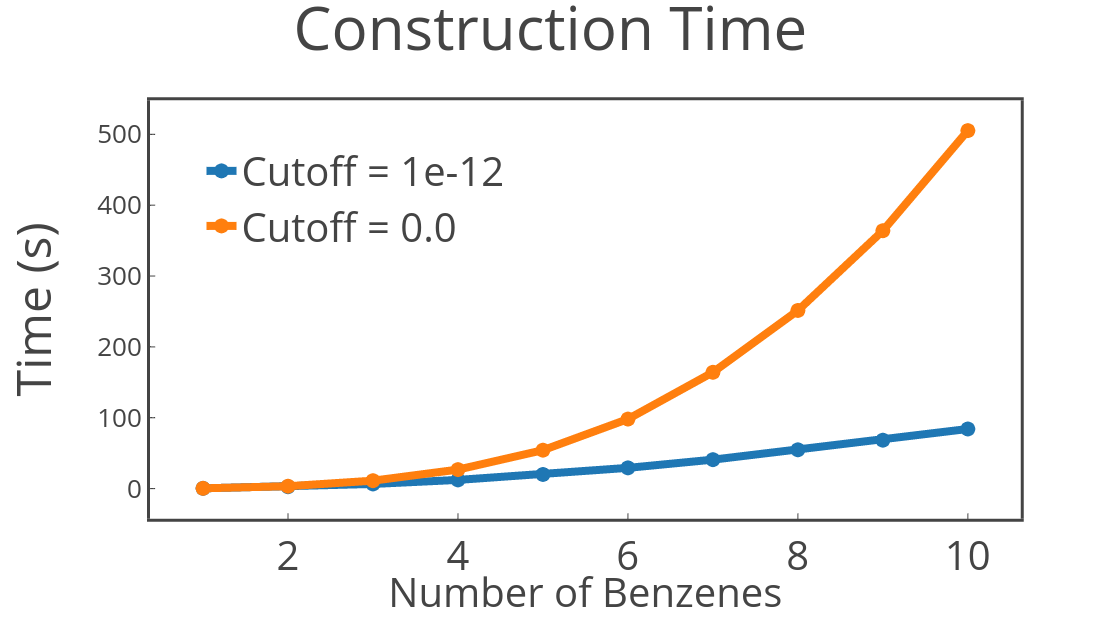
\includegraphics[width=0.5\textwidth]{figures/sparsity_plots/construction_wall.png}\label{fig:f1}}
  \hfill
  \subfloat[]{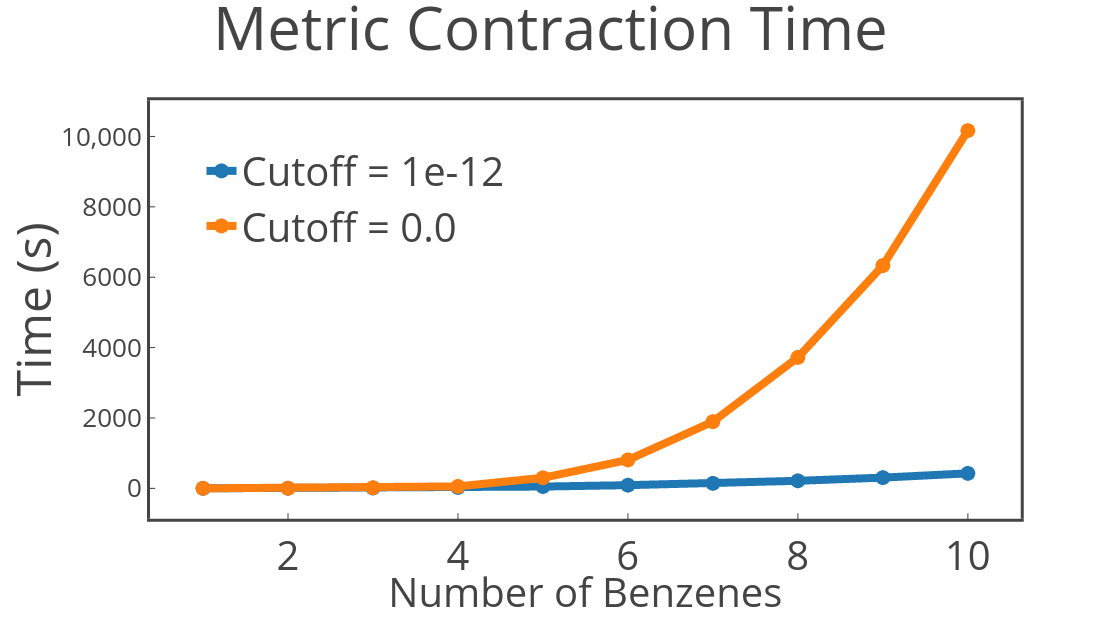
\includegraphics[width=0.5\textwidth]{figures/sparsity_plots/metric_contraction.png}\label{fig:f1}}
  \hfill \\
  \subfloat[]{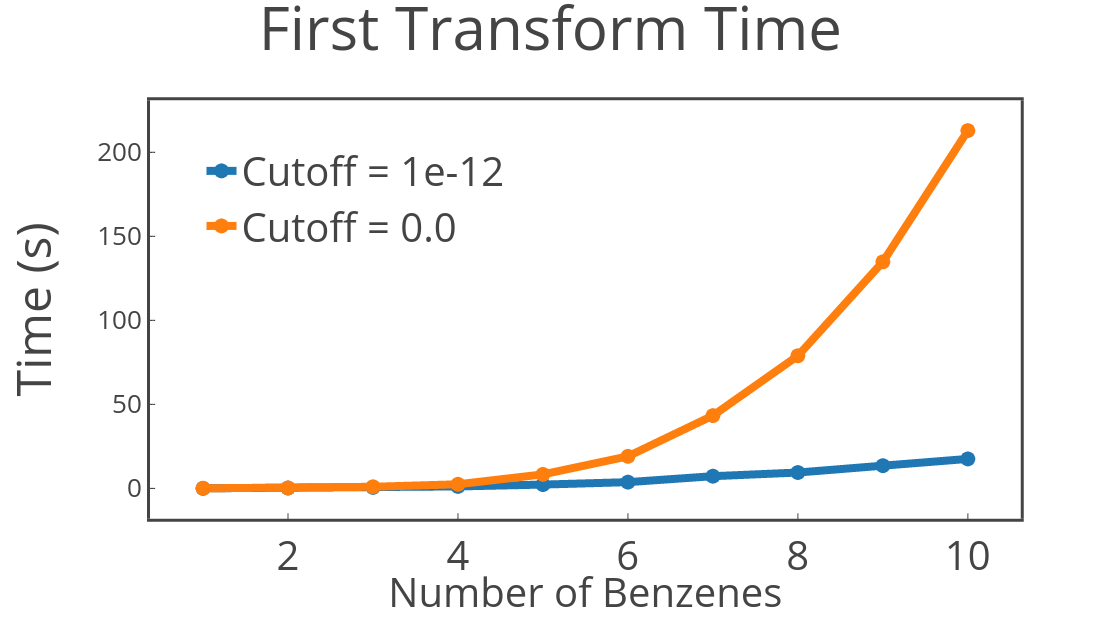
\includegraphics[width=0.5\textwidth]{figures/sparsity_plots/first_transform_wall.png}\label{fig:f1}}
  \hfill
  \subfloat[]{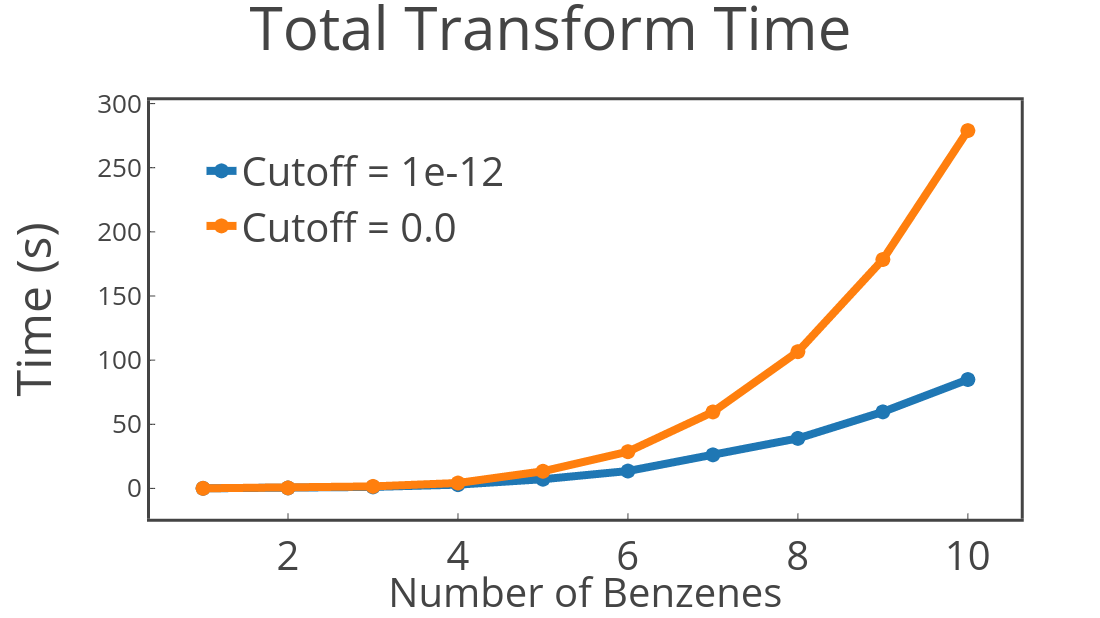
\includegraphics[width=0.5\textwidth]{figures/sparsity_plots/total_transform_wall.png}\label{fig:f2}}
  \caption{Comparison of execution times using sparsity screening (blue) against no sparsity screening (orange).  Execution time is plotted against number of benzenes
 in a benzene stack from one to ten benzenes. Transformations involved computing $(ib|Q)$, where $i$ and $b$ denote occupied and virtual indices, respectively.
 Cutoff refers to the Schwarz screening threshold. (a) Computing the integrals. (b) Contracting AO integrals with the fitting metric. 
(c) first transformation times only. (d) total transformation times.}
\end{figure}

\begingroup
\begin{table}[H]
\centering
\renewcommand{\baselinestretch}{1}
\caption{Speedups obtained from sparsity screening at ten benzenes from data in Figure 2.}
\begin{tabular}{l c}
\multicolumn{1}{l}{\textbf{Operation}} &
\multicolumn{1}{c}{\textbf{Speedup at 10 benzenes}} \\ 
\hline
Construction          & 10.6  \\          
Metric Contraction    & 37.8  \\          
First Transformation  & 25.8  \\          
Total Transformation  & 5.5  \\          
\end{tabular}
\end{table}
\endgroup


Clearly, Figure 2 reveals significant time reductions for all procedures measured.
Table 3 reinforces that operations with higher complexity scaling have the largest time
reduction, with the caveat that total transformation time includes portions without sparsity utilization.
In the integral computations (Figure 2 (a)), we construct the sparse integrals using
function screening; however, we still compute them in shell triplets for effeciency.
Therefore the acquired speedup is slightly less dramatic compared to the metric contraction and
transformation procedures (Figure 2 (b) and (c), respectively) due to select functions being 
screened in cases where the entire shell is not screened. 
Note that the metric contraction is by far the most expensive operation, which should in one part
highlight the boon of sparsity utilization and in another part
illustrate the pertinence of our workflow investigation later in this paper.
Last, our proposal outlined in Algorithm 2 for applying sparsity screening to integral transformations
is proven viable by Figure 2 (c).  Note that significant reductions are obtained for the
first transformation; however, the sparsity thereafter is unrelated to the initial sparsity
mask. With sparsity utilization, the first step scales as $\mathcal{O}(N_{aux}N_{AO}^{1-2}p)$,
whereas the second transformation step will still scale as $\mathcal{O}(N_{aux}N_pN_q)$.
In this work we have not gone on to consider sparsity of the MO indices, which would 
typically require transformation to local orbitals.


\section{Parallel Scaling of Transformations}

To measure parallel scaling, we performed integral transformations for the boron catalyst system shown in Figure 3. 
We varied the problem size by adjusting the $\zeta$ level for the Dunning basis sets with $\zeta$ = D, T, Q.
The characteristics of these systems are included in Table 4. Note that while parallel scaling typically improves
for larger systems (i.e. due to larger workloads),
this is not gauranteed in a sparsity regime. Larger systems may contain more sparsity;
more sparsity will result in more striding, copying, and irregular sizing,
which will hinder parallel scaling. Nonetheless, our method outlined in Algorithm 2 is designed to utilize sparsity while also
obtaining maximum parallel efficiency. 

\begin{figure}[H] 
\centering
\includegraphics[width=80mm]{geometries/boron_catalyst.png} \caption{Transition state for organoboron addition to trifluooroacetone. Taken from Ref. \cite{Lec:2016:768}} 
\label{fig:databases} \end{figure}

\begingroup
\begin{table}[H]
\centering
\renewcommand{\baselinestretch}{1}
\caption{Characteristics of organoboron catalyst.
$N$ and $N_{aux}$ refer to the number of primary and auxiliary basis functions, respectively.
Mask sparsity refers to the percentage of significant AO function pairs in the sparsity mask.}
\begin{tabular}{l ccc}
\multicolumn{1}{l}{\textbf{Basis}} &
\multicolumn{1}{c}{\textbf{$N$}} &
\multicolumn{1}{c}{\textbf{$N_{aux}$}} &
\multicolumn{1}{c}{\textbf{Mask Sparsity (\%)}} \\
\hline
cc-pVDZ   & 671  & 3277 & 29.6 \\          
cc-pVTZ   & 1566 & 3856 & 41.1 \\          
cc-pVQZ   & 3040 & 5593 & 50.2 \\          
\end{tabular}
\end{table}
\endgroup

\noindent For each system, we performed the three common transformations:

\begin{align} 
(i j | Q) = (\lambda \sigma | Q) C_{\sigma i} C_{\lambda j} \\
(i b | Q) = (\lambda \sigma | Q) C_{\sigma i} C_{\lambda b} \\
(a b | Q) = (\lambda \sigma | Q) C_{\sigma a} C_{\lambda b} 
\end{align}

\noindent The experiment was carried out using one node consisting of an Intel Xeon E5-2630 processor 
(10 cores at 2.20GHz) and 24GB DRAM. Figure 4 includes plots of both speedups and execution times for each system.

\begin{figure}[H]
  \centering
  \subfloat[]{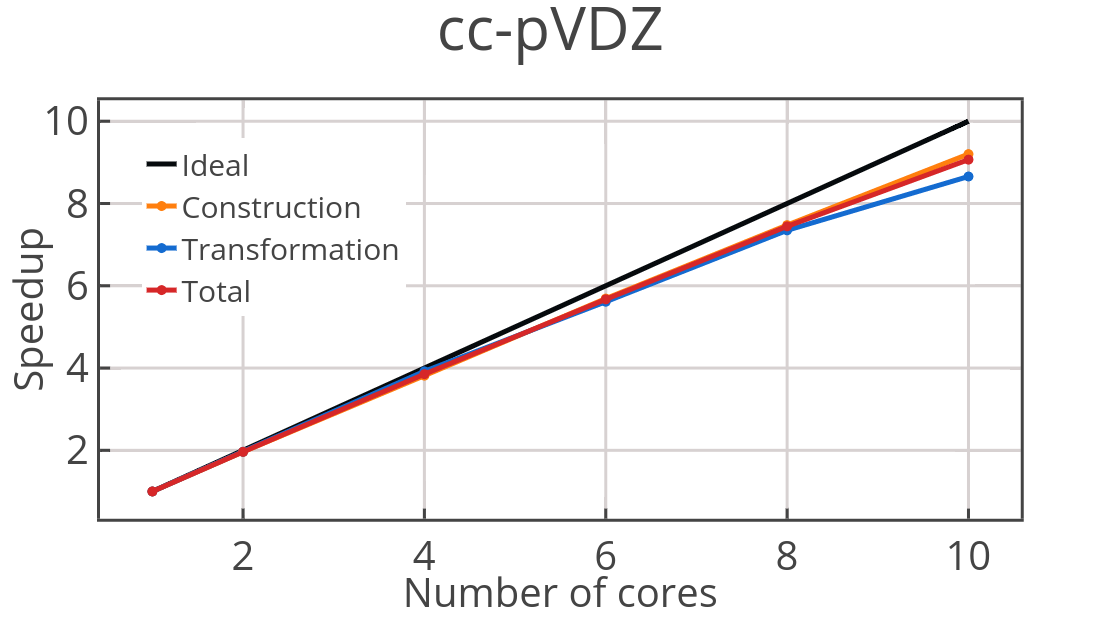
\includegraphics[width=0.5\textwidth]{figures/parallel_scaling_plots/speedup-cc-pVDZ.png}\label{fig:f1}}
  \hfill
  \subfloat[]{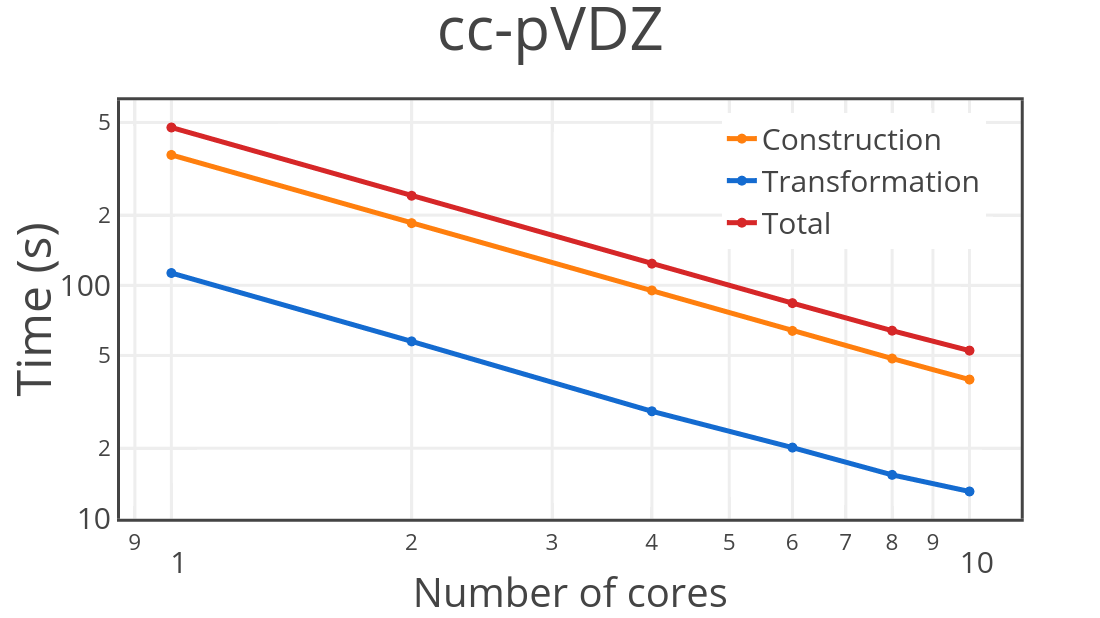
\includegraphics[width=0.5\textwidth]{figures/parallel_scaling_plots/times-cc-pVDZ.png}\label{fig:f2}}
  \hfill
  \subfloat[]{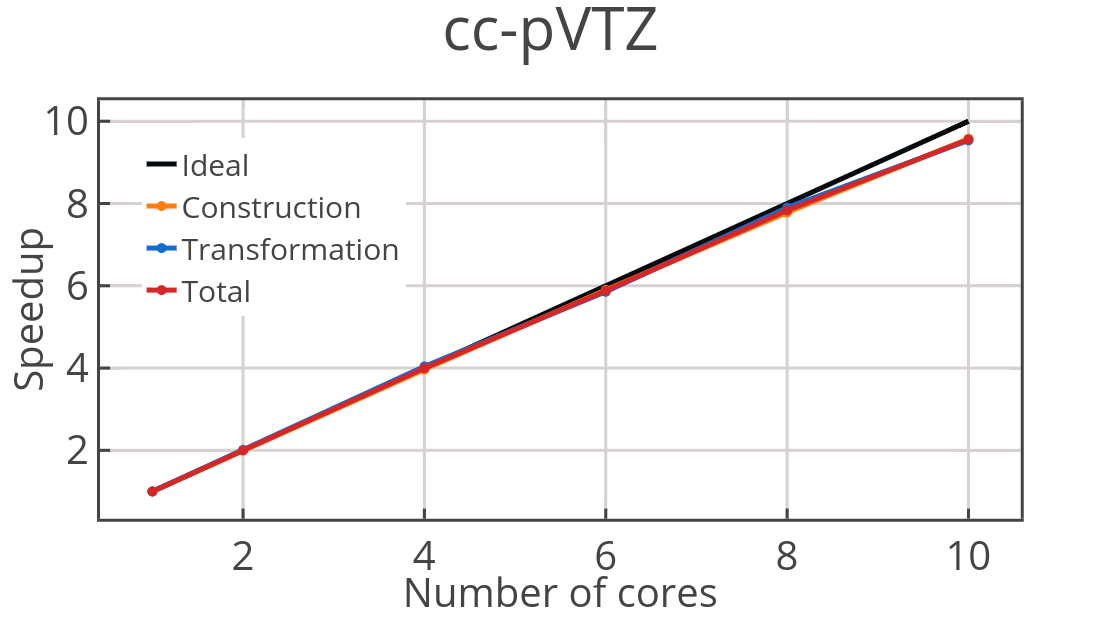
\includegraphics[width=0.5\textwidth]{figures/parallel_scaling_plots/speedup-cc-pVTZ.png}\label{fig:f1}}
  \hfill
  \subfloat[]{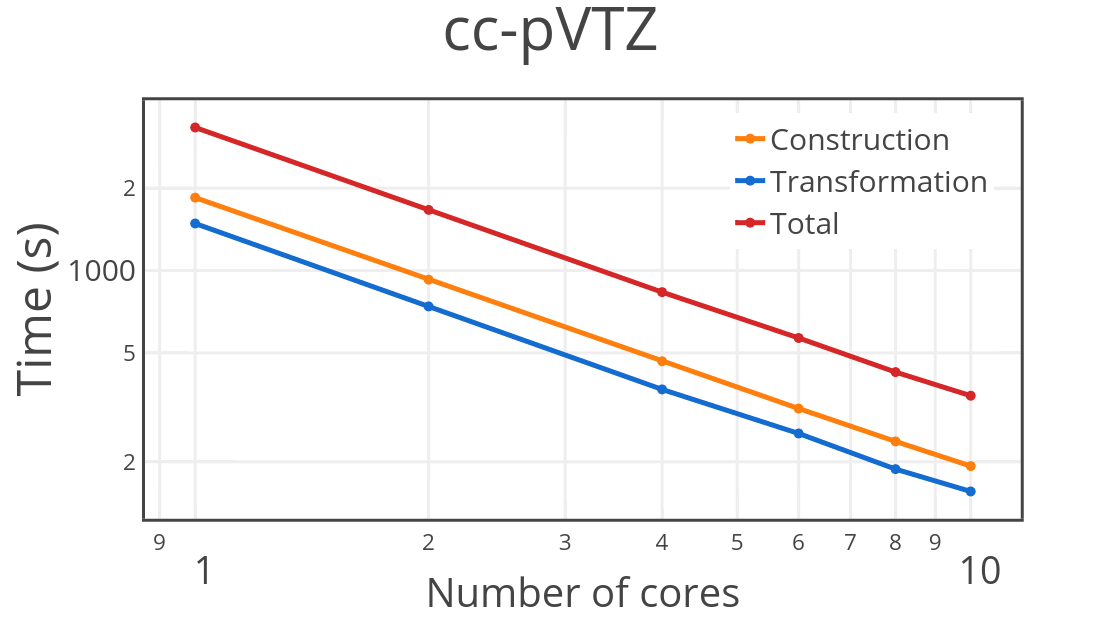
\includegraphics[width=0.5\textwidth]{figures/parallel_scaling_plots/times-cc-pVTZ.png}\label{fig:f2}}
  \hfill
  \subfloat[]{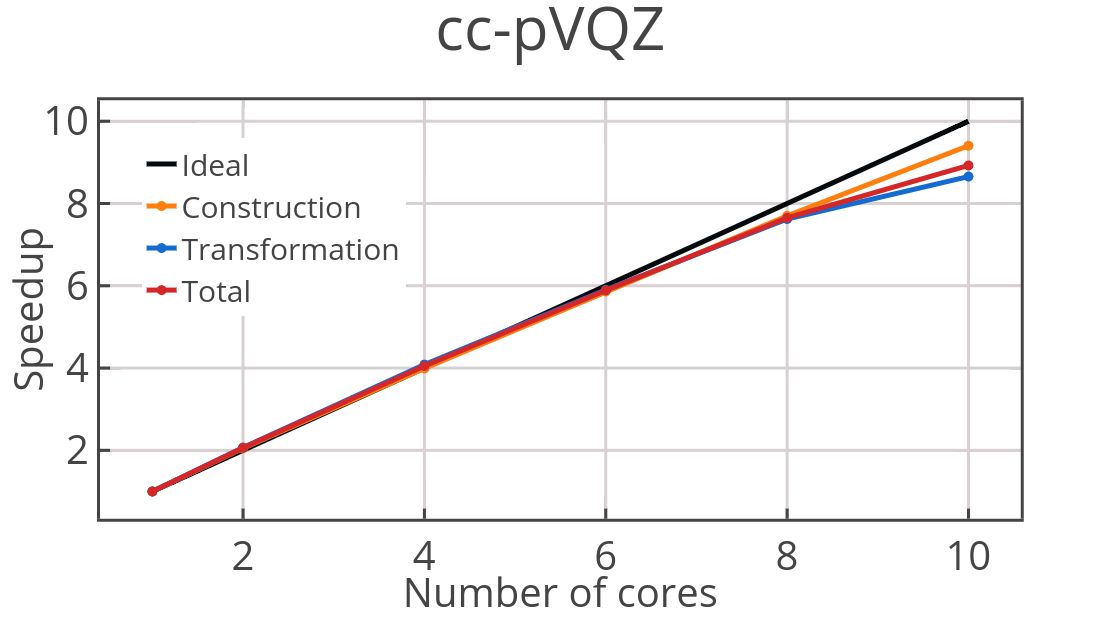
\includegraphics[width=0.5\textwidth]{figures/parallel_scaling_plots/speedup-cc-pVQZ.png}\label{fig:f1}}
  \hfill
  \subfloat[]{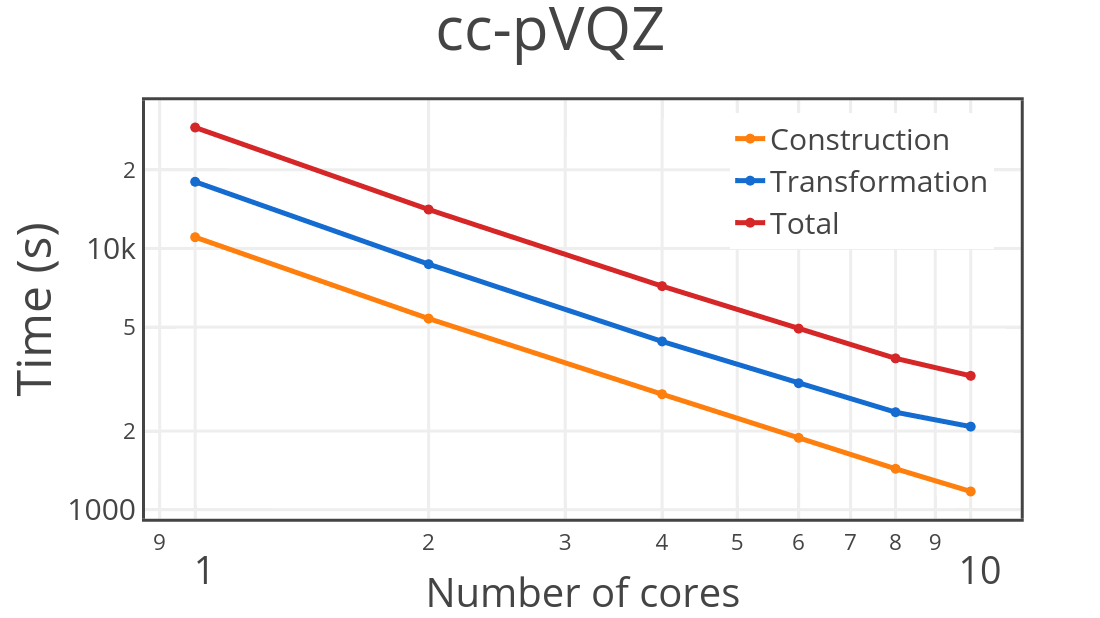
\includegraphics[width=0.5\textwidth]{figures/parallel_scaling_plots/times-cc-pVQZ.png}\label{fig:f2}}
  \hfill
  \caption{Speedup and execution time plots obtained using our optimized memory layout from Section 3 for sparsity screened 3-center integrals. 
 Execution times involve computing three common transformations: $(ij|Q)$, $(ib|Q)$, and $(ab|Q)$,
 where $i,j$ and $a,b$ denote occupied and virtual indices, respectively. Graphs (a), (c), and (e) include speedups for constructing the integrals (orange),
 transforming (blue), total time (red), and ideal (black). Graphs (b), (d), and (f) plot total execution times. Problem sizes were increased by increasing basis set size
 using cc-pVXZ, X = D,T,Q.}
\end{figure}

At ten cores, speedups for total computation time were recorded as 9.09, 9.56, and 8.93 for $\zeta = $ D, T, Q, 
respectively. The improvement in scaling between $\zeta = $ D to $\zeta = $ T
may be attributed to larger system sizes. The sizes of the sparsity screened AO integrals were 10.38GB and 55.70GB 
for these systems, respectively. In the latter case,
the 24GB of memory at the compute node was fully used and work for each thread was increased to maximal levels. Conversely, 
when the system size was increased again using
$\zeta = $ Q, the memory contraint did not allow for further increase in work per thread. 
The hindrance in scaling from $\zeta = $ T to $\zeta = $ Q is explained by the workload inbalance incurred by
the increase in sparsity. 


\section{Context Dependent Workflows}

\subsection{Performace Crossover Through Number of Iterations}
 In this section, we reveal the contexts in which either the Store or Direct algorithms are superior. First, we analyzed performance when applying either algorithm
 to carry out each of the three common integral transformations: $(Q|ij)$, $(Q|ib)$, and $(Q|ab)$. Doing so reveals the crossover in computational complexity that occurs between the two
 algorithms. For few transformations, the Direct algorithm will be superior as it benefits from the speedups given
 in Table 1. However, if many transformations occur, we propose the Store algorithm will become superior as it avoids the costly metric contraction for each transformation.
 
We applied both algorithms to each transformation using the
same boron catalyst system in Section 6.2. To reveal the crossover in computational work between the two algorithms, 
the execution times to carry out one to ten transformations were recorded. To reveal additional trends, we varied the
system size by adjusting the basis set size using $\zeta$ = D, T, Q. The characteristics of these systems are described in Table 5.
The experiments were carried out using one node consisting of an Intel Core i7-5930K processor
(6 cores at 3.50GHz) and 50GB DRAM. The results are plotted in Figure 5.
 
\begingroup
\begin{table}[H]
\centering
\renewcommand{\baselinestretch}{1}
\caption{Characteristics of organoboron catalyst systems across the cc-pVDZ, cc-pVTZ, and cc-pVQZ basis sets.}
\begin{tabular}{l cccc}
\multicolumn{1}{l}{\textbf{Basis}} &
\multicolumn{1}{c}{\textbf{$N$}} &
\multicolumn{1}{c}{\textbf{$N_{aux}$}} &
\multicolumn{1}{c}{\textbf{$N_{occ}$}} &
\multicolumn{1}{c}{\textbf{$N_{virt}$}} \\
\hline
cc-pVDZ   & 671  & 3277      & 129       & 542        \\ 
cc-pVTZ   & 1566 & 3856      & 129       & 1437       \\ 
cc-pVQZ   & 3040 & 5593      & 129       & 2911       \\ 
\end{tabular}
\end{table}
\endgroup

\begin{figure}[H]
  \captionsetup[subfigure]{labelformat=empty}
  \centering
  \subfloat[]{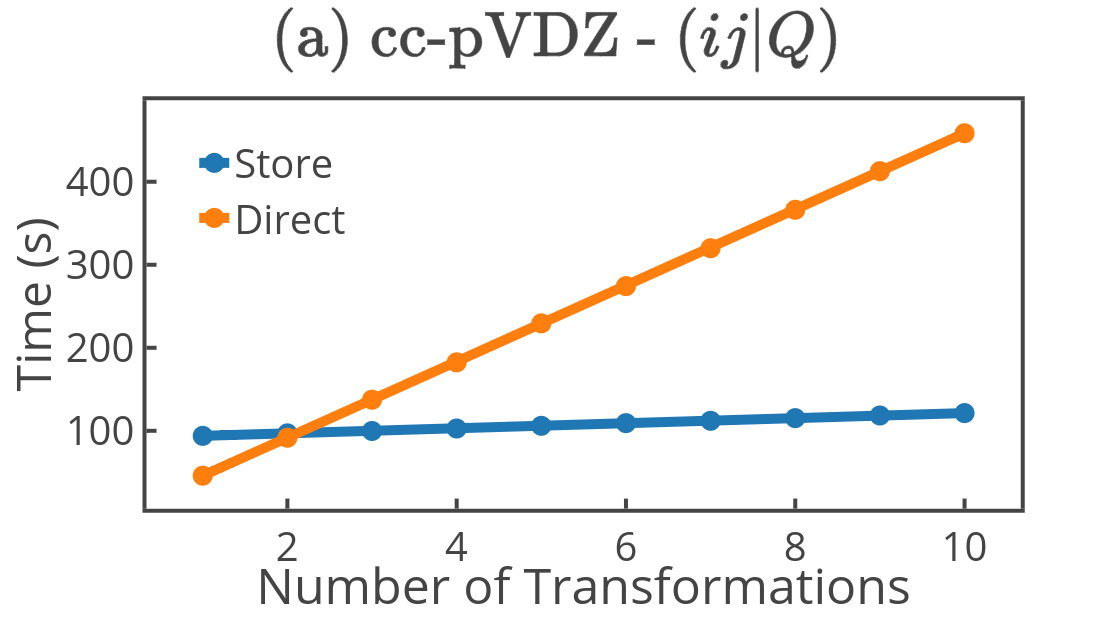
\includegraphics[width=0.35\textwidth]{figures/workflow_plots/input1-cc-pVDZ.png}}
  %\hfill
  \subfloat[]{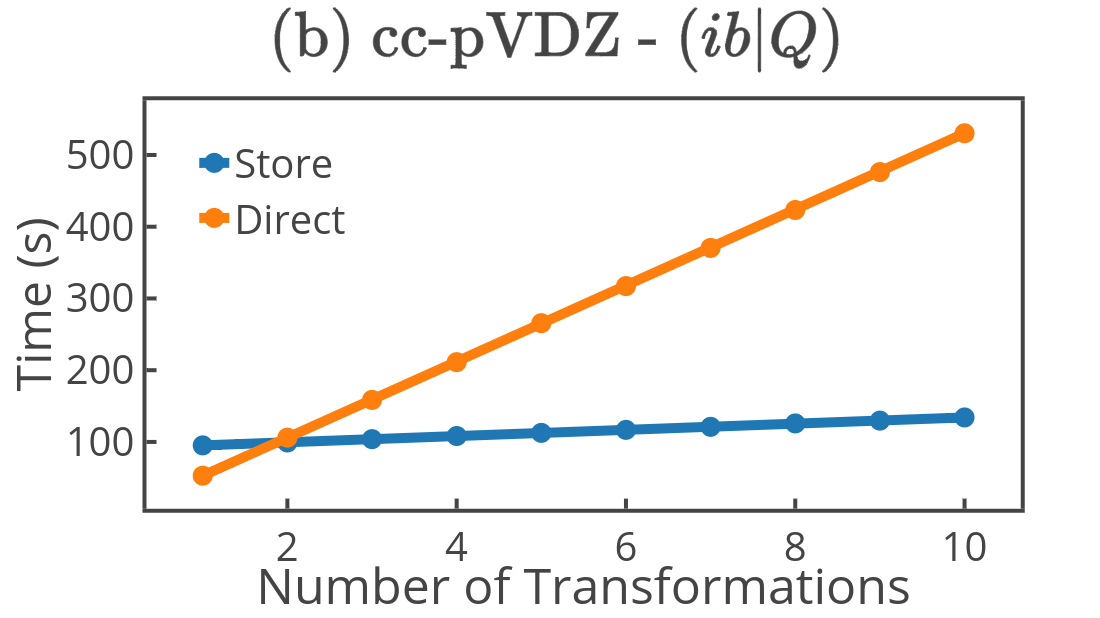
\includegraphics[width=0.35\textwidth]{figures/workflow_plots/input2-cc-pVDZ.png}}
  %\hfill
  \subfloat[]{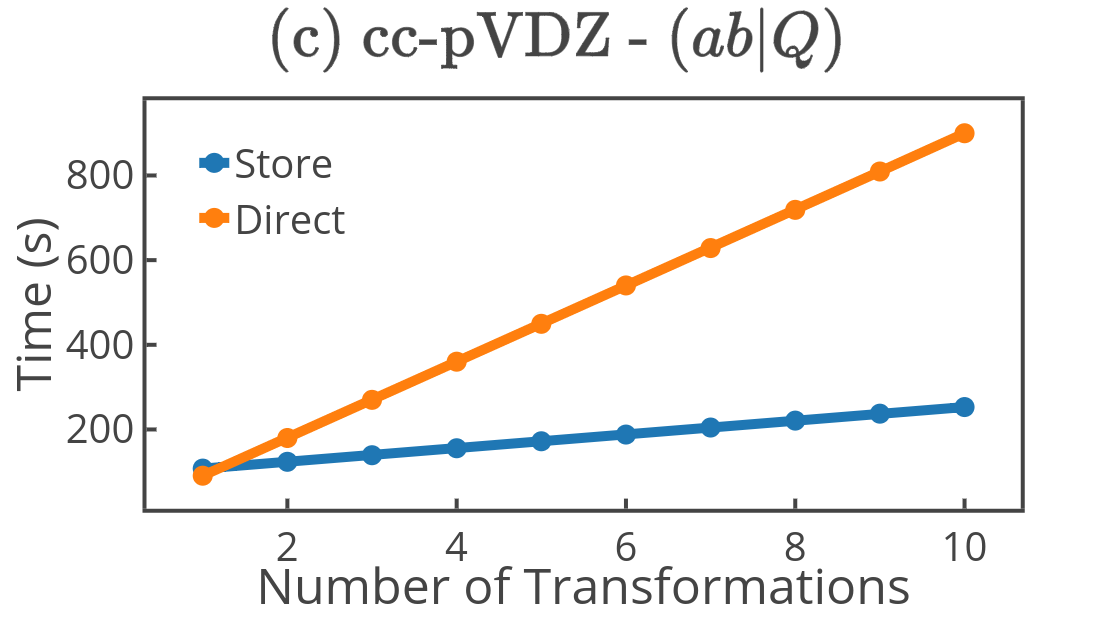
\includegraphics[width=0.35\textwidth]{figures/workflow_plots/input3-cc-pVDZ.png}}\\[-4ex]
  \hfill
  \subfloat[]{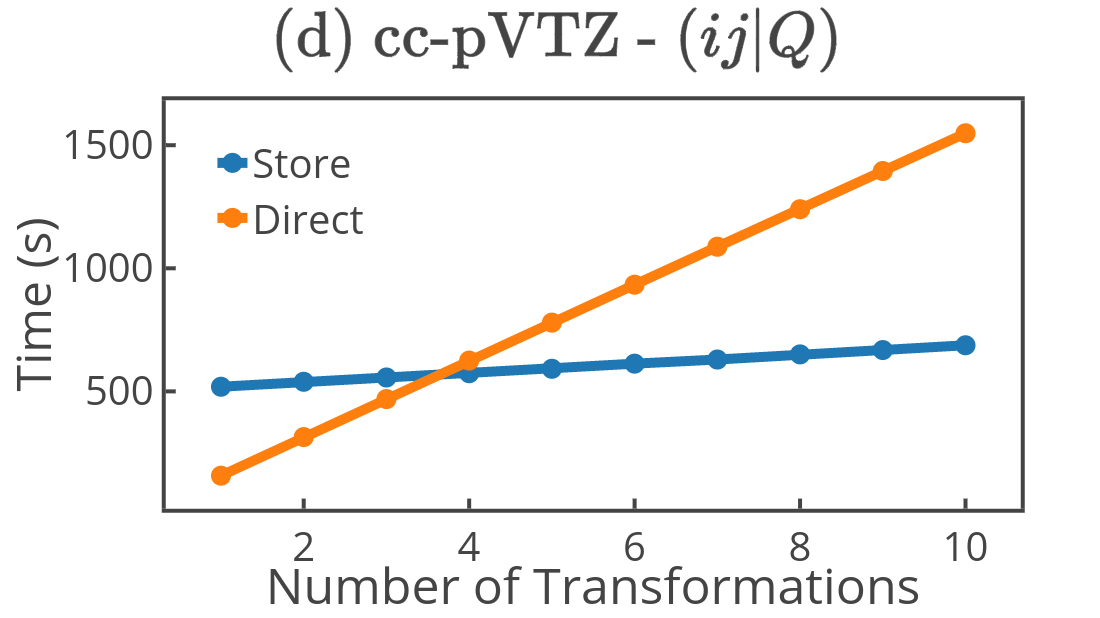
\includegraphics[width=0.35\textwidth]{figures/workflow_plots/input1-cc-pVTZ.png}}
  %\hfill
  \subfloat[]{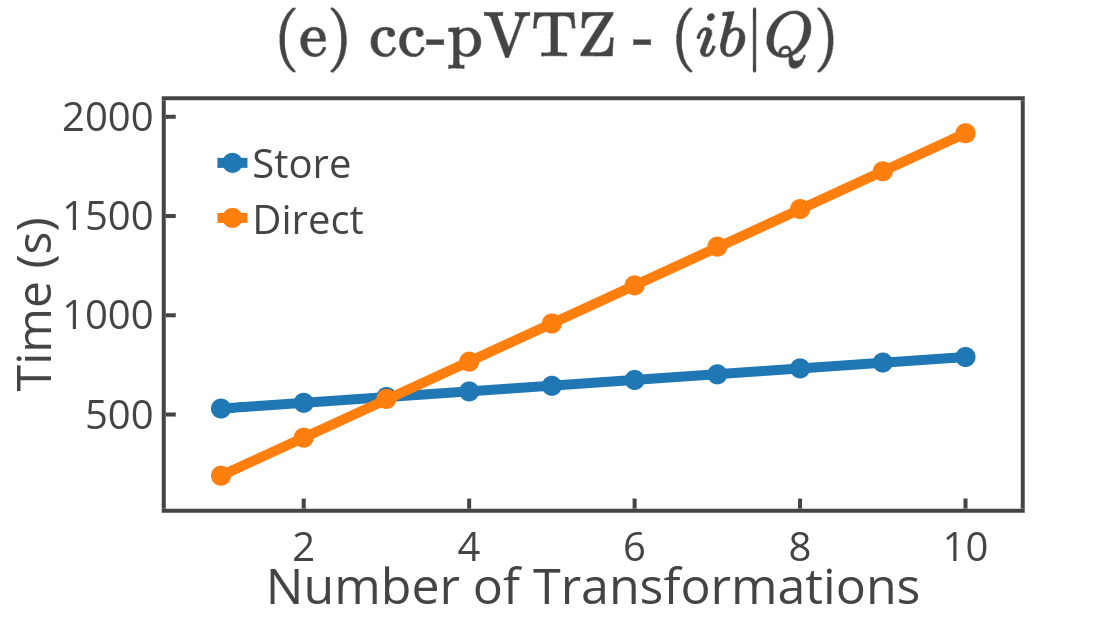
\includegraphics[width=0.35\textwidth]{figures/workflow_plots/input2-cc-pVTZ.png}}
  %\hfill
  \subfloat[]{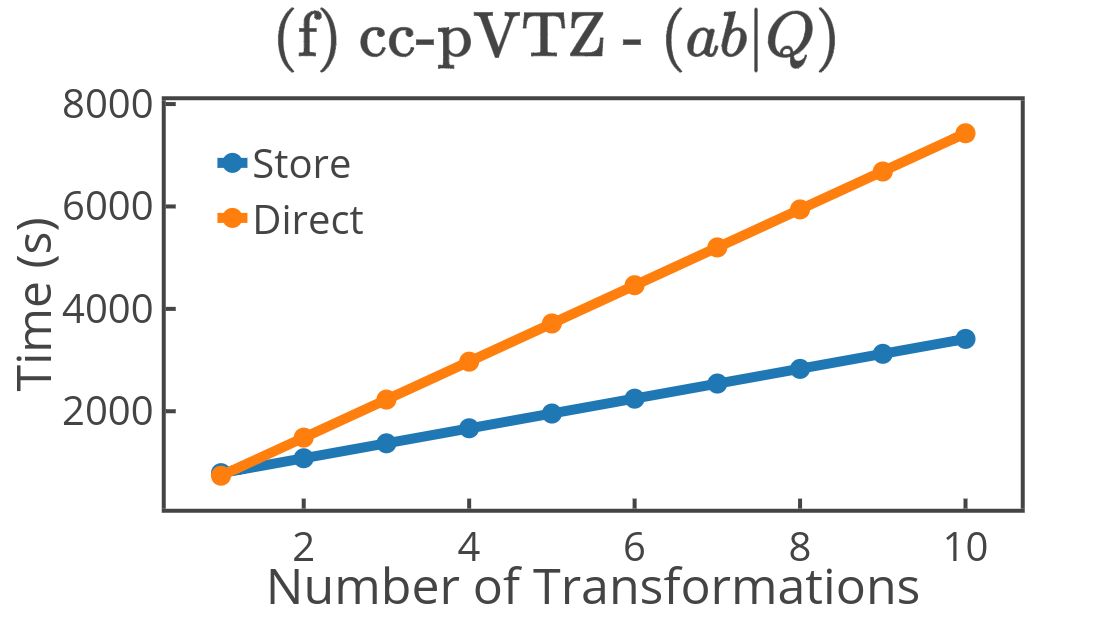
\includegraphics[width=0.35\textwidth]{figures/workflow_plots/input3-cc-pVTZ.png}}\\[-4ex]
  \hfill
  \subfloat[]{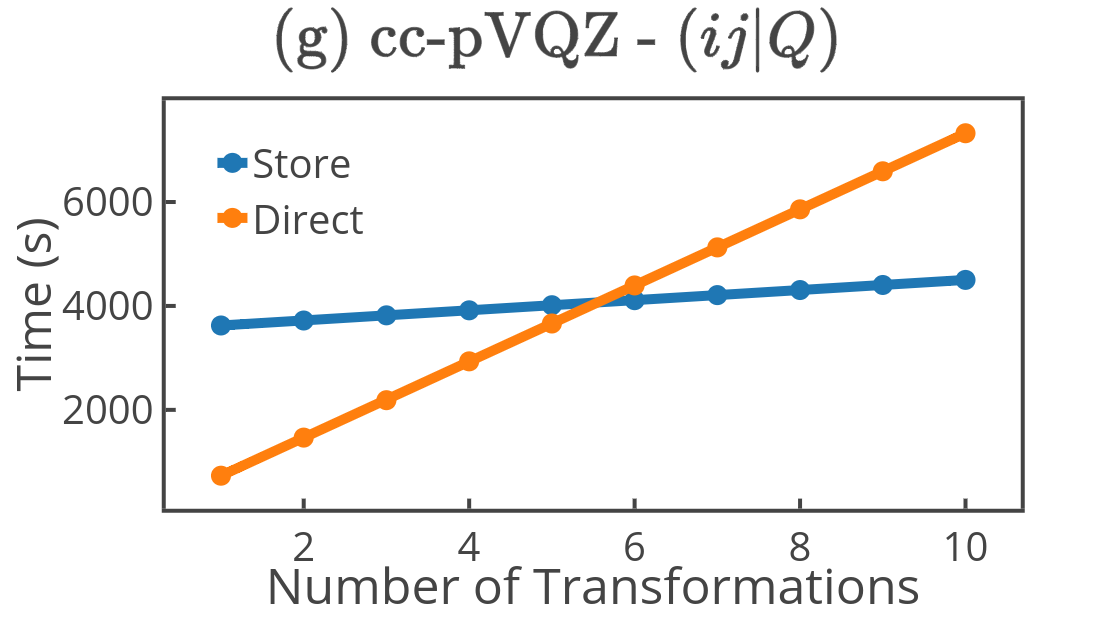
\includegraphics[width=0.35\textwidth]{figures/workflow_plots/input1-cc-pVQZ.png}}
  %\hfill
  \subfloat[]{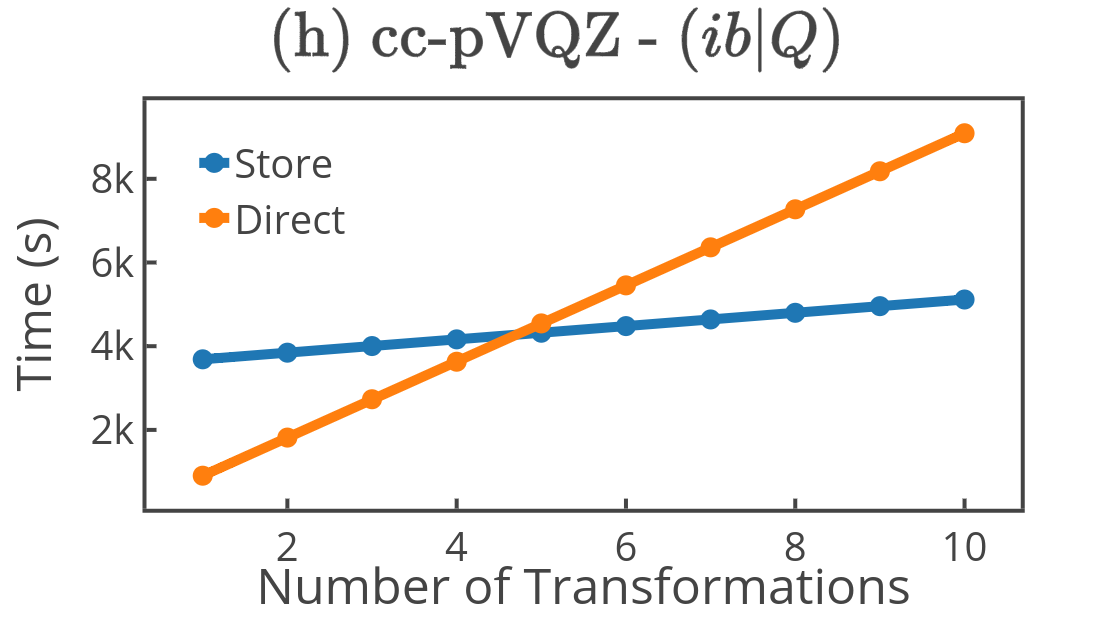
\includegraphics[width=0.35\textwidth]{figures/workflow_plots/input2-cc-pVQZ.png}}
  %\hfill
  \subfloat[]{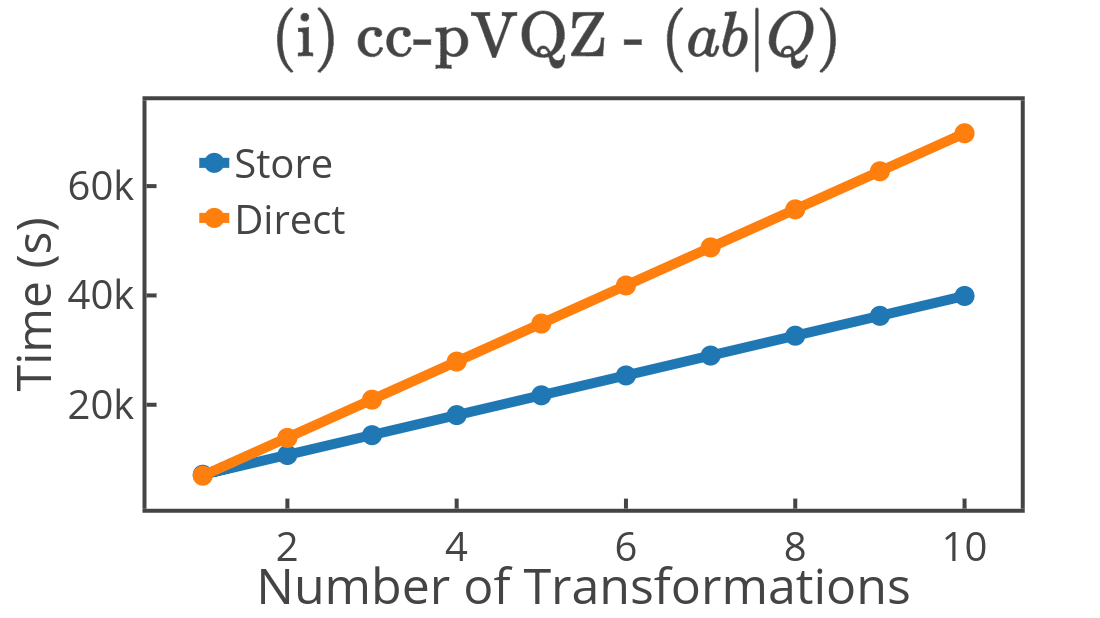
\includegraphics[width=0.35\textwidth]{figures/workflow_plots/input3-cc-pVQZ.png}}
  \caption{Comparison of execution times for the Store and Direct algorithms to complete $(ij|Q)$, $(ib|Q)$, and $(ab|Q)$ transformations
across the cc-pVDZ, cc-pVTZ, and cc-pVQZ basis sets. A scan from one to ten transformations was performed. In each case, a crossover
occurs as the Direct algorithm becomes more expensive. The crossover occurs in fewer iterations for transformations involving larger MO spaces.
With increasing basis set size, the crossover point is shifted to the right for the $(ij|Q)$ and $(ib|Q)$
transformations and it is shifted slightly to the left for the $(ab|Q)$ transformation.}
\end{figure}

If only one transformation occurs, then the speedups of Table 1 enable the Direct algorithm to be superior. 
However, the Direct algorithm must carry out expensive metric contractions for every transformation. As the
number of transformations increase, the expense of these contractions
overtakes the speedups of pre-transforming the integrals. Note that a crossover between the two algorithms occurs in each system. 
This finding supports our conjecture that the Store algorithm is advantageous in contexts where many transformations occur. 
This includes iterative methods where the transformations
are carried out in each iteration, such as MCSCF, as well as methods which require many transformations, such as FSAPT and 
USAPT. Conversely, the Direct algorithm is advantageous for methods
requiring few transformations, such as DFMP2.

Additionally, the crossover point shifts to the left as the transformation spaces get larger ($ij, ia, ab$), occuring in fewer transforamtions.
This finding is supportive of the proposed speedups in Table 1.
Therefore procedures using anything larger than a $(ib|Q)$ transformation will recieve nominal benefits from employing the 
Direct algorithm and may incur slowdowns if many transformations occur.
Last, the crossover point shifts to the right for the $(ij|Q)$ and $(ib|Q)$ transformations as larger basis sets are used. 
This will allow for 
continued benefits with more transformations. Conversely, the crossover shifts to the left for the $(ab|Q)$ transformation
for larger basis sets. Either of these findings are elucidated
by the increasing ratio of $\frac{N_{aux}}{N_{AO}}$. 
 
\subsection{Superior Workflows in Practice}

In the previous section, we determined the Direct algorithm will be superior in methods such as DFMP2, while the Store 
algorithm will be superior in methods such as MCSCF.
After determing the contexts in which either algorithm prevail, we sought to reveal their benefits when applied in practice. 
To do so, we employed either algorithm
in the contexts of different procedures and systems.  For procedures, we tested DFMCSCF and DFMP2.  We ran these 
procedures on the systems included in Figure 5.5.
Figure 5.5 (a) is a hexatriene molecule.  Figure 5.5 (b) is benzene and toluene solvated by 20 water molecules.
Table 5.5 lists the characteristics of each system,
which includes the basis set, the number of primary and auxiliary basis functions, and the mask sparsity. 


\begin{figure}[H]
  \captionsetup[subfigure]{}
  \centering
  \subfloat[]{\includegraphics[width=55mm]{geometries/hexatriene.png}}
  \subfloat[]{\includegraphics[width=55mm]{geometries/benzene-toluene-solvated.png}} 
  \hfill
  \caption{Systems used for context dependent investigation of the Store and Direct workflows. (a) Hexatriene. (b) Benzene and toluene 
in 20 water solvent molecules. }
\end{figure}

\begingroup
\begin{table}[H]
\centering
\renewcommand{\baselinestretch}{1}
\caption{Characteristics of systems for Store vs Direct algorithm comparisons.}
\begin{tabular}{l cccc}
\multicolumn{1}{l}{\textbf{System}} &
\multicolumn{1}{c}{\textbf{Basis}} &
\multicolumn{1}{c}{\textbf{$N_{aux}$}} &
\multicolumn{1}{c}{\textbf{$N_{occ}$}} &
\multicolumn{1}{c}{\textbf{$N_{virt}$}} \\
\hline
Hexatriene        & cc-pVQZ     & 3277      & 129       & 542        \\ 
Benzene-Toluene   & jun-cc-pVDZ & 3856      & 129       & 1437       \\ 
\end{tabular}
\end{table}
\endgroup

The experiments were carried out using one node consisting of an Intel Core i7-5930K processor
(6 cores at 3.50GHz) and 60GB DRAM. The results are included in Tables 5.6 and 5.7. Table 5.6 includes
the total computation time spent in operations involving the three-index integrals. These times will
reflect the algorithmic benifits illustrated in Table 5.4. Table 5.7 includes the total time required
to exectue the program. These times reflect total procedure times, which include many operations extraneous
to the three-index integrals.

\begingroup
\begin{table}[H]
\centering
\renewcommand{\baselinestretch}{1}
\caption{Computatoinal times comparing the Direct and Store algorithms for three-index integral transformations}
\begin{tabular}{l cccc}
\multicolumn{1}{l}{\textbf{System}} &
\multicolumn{1}{c}{\textbf{Procedure}} &
\multicolumn{1}{c}{\textbf{DIRECT}} &
\multicolumn{1}{c}{\textbf{STORE}} &
\multicolumn{1}{c}{\textbf{Speedup}} \\ 
\hline
Hexatriene        & DFMCSCF & 42.32s  & 7.839s  &  5.4x  \\ 
Hexatriene        & DFMP2   & 2.728s  & 6.559s  &  2.4x  \\ 
Benzene-Toluene   & DFMCSCF & 438.1s  & 104.8s  &  4.2x  \\ 
Benzene-Toluene   & DFMP2   &      &   &    \\ 
\end{tabular}
\end{table}
\endgroup


\begingroup
\begin{table}[H]
\centering
\renewcommand{\baselinestretch}{1}
\caption{Total procedure wall clock times comparing the Direct and Store algorithms for three-index integral transformations}
\begin{tabular}{l cccc}
\multicolumn{1}{l}{\textbf{System}} &
\multicolumn{1}{c}{\textbf{Procedure}} &
\multicolumn{1}{c}{\textbf{DIRECT}} &
\multicolumn{1}{c}{\textbf{STORE}} &
\multicolumn{1}{c}{\textbf{Speedup}} \\ 
\hline
Hexatriene        & DFMCSCF & 173.0   & 145.6   &  1.2x  \\ 
Hexatriene        & DFMP2   & 1299.4s & 1307.3s &  1.0x  \\ 
Benzene-Toluene   & DFMCSCF & 5138.7s & 4811.8s &  1.1x  \\ 
Benzene-Toluene   & DFMP2   &   &   &    \\ 
\end{tabular}
\end{table}
\endgroup

Both Tables 5.6 and 5.7 reveal that the Direct algorithm is superior for DFMP2 whereas the Store algorithm is superior for
DFMCSCF. The computational speedups can be substantial, reaching 5.4x for DFMCSCF with the hexatriene system. However, Table 5.7
reveals these speedups are considerably dampened for the overall procedure time. This is true because 
the operations invovling the three-index integrals ar enot the most expensive compoutations occurring within these procedures.


\section{Coloumb and Exchange Builds}

Here, we present the performance of Algorithms 10 and 11 for various systems. Currently, the state of the art in the 
open-source electronic structure package, Psi4, is Algorithm 11. However, we conjecture that Algorithm 10 could provide 
considerable speedups as it eliminates entirely a strided, level 1 BLAS copy.   

We implemented Algorithm 10 and incorporated it into a development version of Psi4. Then, we used Psi4's Self-Consistent-Field
procedure to produce energies for various systems and basis set combinations. The systems used involved a protein-drug complex,
where the drug molecule is ommitted and the atoms of the protien are added in a series according to distance from the center of
the drug molecule. 

The experiments were carried out using one node consisting of an Intel Core i7-5930K processor
(6 cores at 3.50GHz) and 60GB DRAM. The results are included in Table 5.7:


 
 



%%%%%%%%%%%%%%%%
% Appendices
%%%%%%%%%%%%%%%%

%\begin{appendices}

%Some Table of Contents entry formatting
\addtocontents{toc}{\protect\renewcommand{\protect\cftchappresnum}{\appendixname\space}}
\addtocontents{toc}{\protect\renewcommand{\protect\cftchapnumwidth}{6em}}

%Begin individual appendices, separated as chapters

\chapter{Experimental Equipment}
Lorem ipsum dolor sit amet, consectetur adipiscing elit, sed do eiusmod tempor incididunt ut labore et dolore magna aliqua. Ut enim ad minim veniam, quis nostrud exercitation ullamco laboris nisi ut aliquip ex ea commodo consequat. Duis aute irure dolor in reprehenderit in voluptate velit esse cillum dolore eu fugiat nulla pariatur. Excepteur sint occaecat cupidatat non proident, sunt in culpa qui officia deserunt mollit anim id est laborum.

\chapter{Data Processing}
Lorem ipsum dolor sit amet, consectetur adipiscing elit, sed do eiusmod tempor incididunt ut labore et dolore magna aliqua. Ut enim ad minim veniam, quis nostrud exercitation ullamco laboris nisi ut aliquip ex ea commodo consequat. Duis aute irure dolor in reprehenderit in voluptate velit esse cillum dolore eu fugiat nulla pariatur. Excepteur sint occaecat cupidatat non proident, sunt in culpa qui officia deserunt mollit anim id est laborum.

\end{appendices}

%%%%%%%%%%%%%%%%
% References
%%%%%%%%%%%%%%%%

\begin{singlespace}  % use single-line spacing for multi-line text within a single reference
	\setlength\bibitemsep{\baselineskip}  %manually set separataion betwen items in bibliography to double space
	\printbibliography[title={References}]
\end{singlespace}

\addcontentsline{toc}{chapter}{References}  %add References section to Table of Contents

\end{document}
